\subsection{Evaluating the single-layer potential: Source points =
target points}
\begin{figure}[htpb]
  \centering
  \begin{tabular}{ccc}
  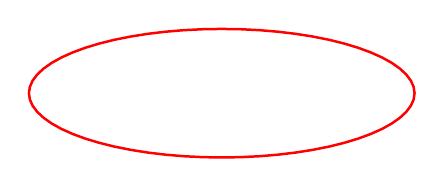
\begin{tikzpicture}[scale=0.6]

\begin{axis}[
  xmin = -3.1,
  xmax = 3.1,
  ymin = -1.1,
  ymax = 1.1,
  scale only axis,
  axis equal image,
  hide axis,
  ]

\addplot [mark=none,red,line width=1.5] table{
3.0000e+00 0.0000e+00
2.9856e+00 9.8017e-02
2.9424e+00 1.9509e-01
2.8708e+00 2.9028e-01
2.7716e+00 3.8268e-01
2.6458e+00 4.7140e-01
2.4944e+00 5.5557e-01
2.3190e+00 6.3439e-01
2.1213e+00 7.0711e-01
1.9032e+00 7.7301e-01
1.6667e+00 8.3147e-01
1.4142e+00 8.8192e-01
1.1481e+00 9.2388e-01
8.7085e-01 9.5694e-01
5.8527e-01 9.8079e-01
2.9405e-01 9.9518e-01
1.8370e-16 1.0000e+00
-2.9405e-01 9.9518e-01
-5.8527e-01 9.8079e-01
-8.7085e-01 9.5694e-01
-1.1481e+00 9.2388e-01
-1.4142e+00 8.8192e-01
-1.6667e+00 8.3147e-01
-1.9032e+00 7.7301e-01
-2.1213e+00 7.0711e-01
-2.3190e+00 6.3439e-01
-2.4944e+00 5.5557e-01
-2.6458e+00 4.7140e-01
-2.7716e+00 3.8268e-01
-2.8708e+00 2.9028e-01
-2.9424e+00 1.9509e-01
-2.9856e+00 9.8017e-02
-3.0000e+00 1.2246e-16
-2.9856e+00 -9.8017e-02
-2.9424e+00 -1.9509e-01
-2.8708e+00 -2.9028e-01
-2.7716e+00 -3.8268e-01
-2.6458e+00 -4.7140e-01
-2.4944e+00 -5.5557e-01
-2.3190e+00 -6.3439e-01
-2.1213e+00 -7.0711e-01
-1.9032e+00 -7.7301e-01
-1.6667e+00 -8.3147e-01
-1.4142e+00 -8.8192e-01
-1.1481e+00 -9.2388e-01
-8.7085e-01 -9.5694e-01
-5.8527e-01 -9.8079e-01
-2.9405e-01 -9.9518e-01
-5.5109e-16 -1.0000e+00
2.9405e-01 -9.9518e-01
5.8527e-01 -9.8079e-01
8.7085e-01 -9.5694e-01
1.1481e+00 -9.2388e-01
1.4142e+00 -8.8192e-01
1.6667e+00 -8.3147e-01
1.9032e+00 -7.7301e-01
2.1213e+00 -7.0711e-01
2.3190e+00 -6.3439e-01
2.4944e+00 -5.5557e-01
2.6458e+00 -4.7140e-01
2.7716e+00 -3.8268e-01
2.8708e+00 -2.9028e-01
2.9424e+00 -1.9509e-01
2.9856e+00 -9.8017e-02
3.0000e+00 0.0000e+00
};

\end{axis}


\end{tikzpicture}

 &
  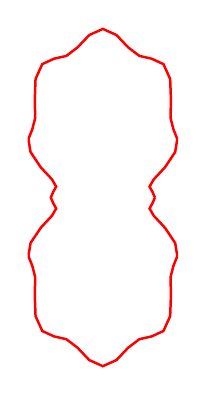
\begin{tikzpicture}[scale=0.6]

\begin{axis}[
  xmin = -0.7,
  xmax = 0.7,
  ymin = -1.6,
  ymax = 1.6,
  scale only axis,
  axis equal image,
  hide axis,
  ]

\addplot [mark=none,red,line width=1.5] table{
4.8450e-01 0.0000e+00
4.6157e-01 5.3483e-02
4.3482e-01 1.0175e-01
4.7362e-01 1.6902e-01
5.7862e-01 2.8197e-01
6.7317e-01 4.2331e-01
6.9318e-01 5.4490e-01
6.5726e-01 6.3458e-01
6.2991e-01 7.4107e-01
6.3378e-01 9.0854e-01
6.2678e-01 1.1036e+00
5.6432e-01 1.2421e+00
4.5506e-01 1.2925e+00
3.4002e-01 1.3187e+00
2.3629e-01 1.3975e+00
1.2667e-01 1.5130e+00
8.1715e-17 1.5700e+00
-1.2667e-01 1.5130e+00
-2.3629e-01 1.3975e+00
-3.4002e-01 1.3187e+00
-4.5506e-01 1.2925e+00
-5.6432e-01 1.2421e+00
-6.2678e-01 1.1036e+00
-6.3378e-01 9.0854e-01
-6.2991e-01 7.4107e-01
-6.5726e-01 6.3458e-01
-6.9318e-01 5.4490e-01
-6.7317e-01 4.2331e-01
-5.7862e-01 2.8197e-01
-4.7362e-01 1.6902e-01
-4.3482e-01 1.0175e-01
-4.6157e-01 5.3483e-02
-4.8450e-01 6.9805e-17
-4.6157e-01 -5.3483e-02
-4.3482e-01 -1.0175e-01
-4.7362e-01 -1.6902e-01
-5.7862e-01 -2.8197e-01
-6.7317e-01 -4.2331e-01
-6.9318e-01 -5.4490e-01
-6.5726e-01 -6.3458e-01
-6.2991e-01 -7.4107e-01
-6.3378e-01 -9.0854e-01
-6.2678e-01 -1.1036e+00
-5.6432e-01 -1.2421e+00
-4.5506e-01 -1.2925e+00
-3.4002e-01 -1.3187e+00
-2.3629e-01 -1.3975e+00
-1.2667e-01 -1.5130e+00
-2.4514e-16 -1.5700e+00
1.2667e-01 -1.5130e+00
2.3629e-01 -1.3975e+00
3.4002e-01 -1.3187e+00
4.5506e-01 -1.2925e+00
5.6432e-01 -1.2421e+00
6.2678e-01 -1.1036e+00
6.3378e-01 -9.0854e-01
6.2991e-01 -7.4107e-01
6.5726e-01 -6.3458e-01
6.9318e-01 -5.4490e-01
6.7317e-01 -4.2331e-01
5.7862e-01 -2.8197e-01
4.7362e-01 -1.6902e-01
4.3482e-01 -1.0175e-01
4.6157e-01 -5.3483e-02
4.8450e-01 0.0000e+00
};

\end{axis}


\end{tikzpicture}

 & 
  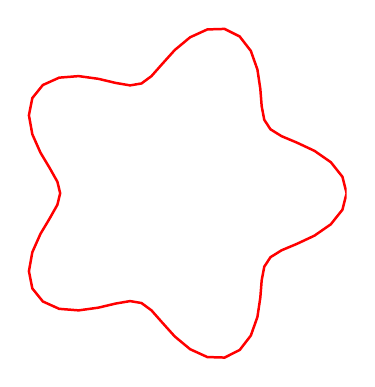
\begin{tikzpicture}[scale=0.6]

\begin{axis}[
  xmin = -1.2,
  xmax = 1.2,
  ymin = -1.2,
  ymax = 1.2,
  scale only axis,
  axis equal image,
  hide axis,
  ]

\addplot [mark=none,red,line width=1.5] table{
1.2000e+00 0.0000e+00
1.1707e+00 1.1531e-01
1.0898e+00 2.1677e-01
9.7570e-01 2.9598e-01
8.5317e-01 3.5339e-01
7.4557e-01 3.9852e-01
6.6837e-01 4.4659e-01
6.2507e-01 5.1298e-01
6.0711e-01 6.0711e-01
5.9756e-01 7.2813e-01
5.7725e-01 8.6391e-01
5.3121e-01 9.9382e-01
4.5339e-01 1.0946e+00
3.4806e-01 1.1474e+00
2.2753e-01 1.1439e+00
1.0726e-01 1.0890e+00
6.1232e-17 1.0000e+00
-8.8776e-02 9.0136e-01
-1.6265e-01 8.1769e-01
-2.3251e-01 7.6647e-01
-3.1197e-01 7.5317e-01
-4.1159e-01 7.7002e-01
-5.3389e-01 7.9903e-01
-6.7122e-01 8.1789e-01
-8.0711e-01 8.0711e-01
-9.2096e-01 7.5581e-01
-9.9457e-01 6.6455e-01
-1.0183e+00 5.4428e-01
-9.9459e-01 4.1197e-01
-9.3818e-01 2.8459e-01
-8.7181e-01 1.7341e-01
-8.1965e-01 8.0728e-02
-8.0000e-01 9.7972e-17
-8.1965e-01 -8.0728e-02
-8.7181e-01 -1.7341e-01
-9.3818e-01 -2.8459e-01
-9.9459e-01 -4.1197e-01
-1.0183e+00 -5.4428e-01
-9.9457e-01 -6.6455e-01
-9.2096e-01 -7.5581e-01
-8.0711e-01 -8.0711e-01
-6.7122e-01 -8.1789e-01
-5.3389e-01 -7.9903e-01
-4.1159e-01 -7.7002e-01
-3.1197e-01 -7.5317e-01
-2.3251e-01 -7.6647e-01
-1.6265e-01 -8.1769e-01
-8.8776e-02 -9.0136e-01
-1.8370e-16 -1.0000e+00
1.0726e-01 -1.0890e+00
2.2753e-01 -1.1439e+00
3.4806e-01 -1.1474e+00
4.5339e-01 -1.0946e+00
5.3121e-01 -9.9382e-01
5.7725e-01 -8.6391e-01
5.9756e-01 -7.2813e-01
6.0711e-01 -6.0711e-01
6.2507e-01 -5.1298e-01
6.6837e-01 -4.4659e-01
7.4557e-01 -3.9852e-01
8.5317e-01 -3.5339e-01
9.7570e-01 -2.9598e-01
1.0898e+00 -2.1677e-01
1.1707e+00 -1.1531e-01
1.2000e+00 0.0000e+00
};

\end{axis}


\end{tikzpicture}


  \end{tabular}
  \mcaption{The three geometries under consideration.}{f:geomsAliasing}
\end{figure}

Here we consider the effect of aliasing when evaluating the Stokes
single- and double-layer potentials
\begin{align*}
  &\SS[\ssigma](\xx) = \frac{1}{4\pi}\int_{\gamma} \left(-\log \rho +
  \frac{\rr \otimes \rr}{\rho^{2}}\right)\ssigma(\yy) ds_{\yy},
  &&\xx \in \gamma, \\
  &\DD[\ssigma](\xx) = \frac{1}{\pi}\int_{\gamma}
  \frac{\rr \cdot \nn}{\rho^{2}}
  \frac{\rr \otimes \rr}{\rho^{2}}\ssigma(\yy) ds_{\yy},
  &&\xx \in \gamma, \\
  &\rr = \xx - \yy, \rho = \|\rr\|,
\end{align*}
where $\nn$ is the unit outward normal and the source and target points
coincide.  If $\gamma$ is discretized with too few points, there are
several operations that will introduce aliasing such as computing the
distance squared $\rho^{2} = (x_{1} - y_{1})^{2} + (x_{2}-y_{2})^2$, and
the product $\ssigma(\yy) |\yy'|$.  Additional terms that result in
aliasing are $\log \rho$ and the Jacobian $|\yy'|$ which requires
computing a square-root.  To see the effect of aliasing, we apply
Alpert's quadrature rules~\cite{alp1999} for the three geometries in
Figure~\ref{f:geomsAliasing}.  We arbitrarily choose the density
function $\ssigma(\theta) = [\exp(\cos \theta),\exp(\cos(\sin
\theta))]$.  A reference solution for each layer potential is formed
using a highly refined grid with 512 points.  In
Figure~\ref{f:aliasingErrors}, we plot the spectrums of the exact and the
approximate single-layer potential, and this reveals the aliasing
errors, especially in the tails of the spectrums.

\begin{figure}[htpb]
  \centering
  \begin{tabular}{ccc}
  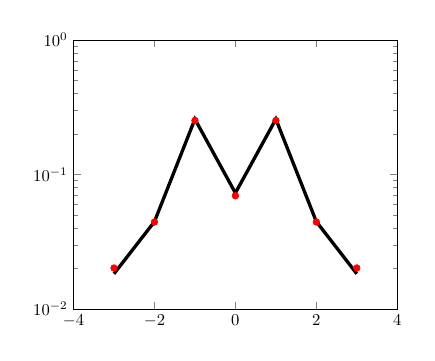
\begin{tikzpicture}[scale=0.6]

\begin{axis}[
  xmin = -4,
  xmax = 4,
  xtick = {-4,-2,0,2,4},
%  xlabel = {Number of Time Steps},
  ymin = 1.0e-2,
  ymax = 1.0e-0,
  ytick = {1e-2,1e-1,1e0},
%  yticklabels = {$10^{-4}$,$10^{-3}$,$10^{-2}$,$10^{-1}$},
  ymode = log,
%  ylabel = {Error},
%  ylabel style = {yshift = 10pt},
%  legend style = {font=\small},
%  legend entries = {no fixes ($N=64$,fix area and length,reduce aliasing,both},
%  legend style = {draw=none},
  ]

% "Exact" single-layer potential
\addplot [color=black,solid,line width=2] table{
-3.0000e+00 1.8265e-02
-2.0000e+00 4.4583e-02
-1.0000e+00 2.5781e-01
0.0000e+00 7.2810e-02
1.0000e+00 2.5781e-01
2.0000e+00 4.4583e-02
3.0000e+00 1.8265e-02
};

% No anti-aliasing; Yes shape correct
\addplot [color=red,only marks,mark=*] table{
-3.0000e+00 2.0166e-02
-2.0000e+00 4.4357e-02
-1.0000e+00 2.5199e-01
0.0000e+00 6.9478e-02
1.0000e+00 2.5199e-01
2.0000e+00 4.4357e-02
3.0000e+00 2.0166e-02
};


\end{axis}


\end{tikzpicture}

 &
  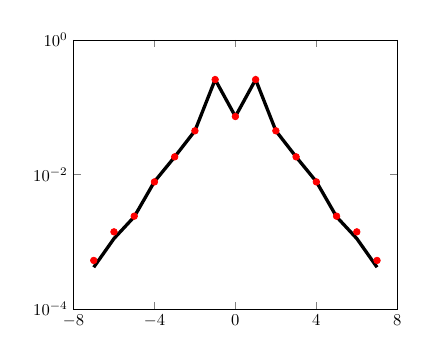
\begin{tikzpicture}[scale=0.6]

\begin{axis}[
  xmin = -8,
  xmax = 8,
  xtick = {-8,-4,0,4,8},
%  xlabel = {Number of Time Steps},
  ymin = 1.0e-4,
  ymax = 1.0e-0,
  ytick = {1e-4,1e-2,1e0},
%  ytick = {1e-4,1e-3,1e-2,1e-1},
%  yticklabels = {$10^{-4}$,$10^{-3}$,$10^{-2}$,$10^{-1}$},
  ymode = log,
%  ylabel = {Error},
%  ylabel style = {yshift = 10pt},
%  legend style = {font=\small},
%  legend entries = {no fixes ($N=64$,fix area and length,reduce aliasing,both},
%  legend style = {draw=none},
  ]

% "Exact" single-layer potential
\addplot [color=black,solid,line width=2] table{
-7.0000e+00 4.1677e-04
-6.0000e+00 1.1132e-03
-5.0000e+00 2.3480e-03
-4.0000e+00 7.8248e-03
-3.0000e+00 1.8265e-02
-2.0000e+00 4.4583e-02
-1.0000e+00 2.5781e-01
0.0000e+00 7.2810e-02
1.0000e+00 2.5781e-01
2.0000e+00 4.4583e-02
3.0000e+00 1.8265e-02
4.0000e+00 7.8248e-03
5.0000e+00 2.3480e-03
6.0000e+00 1.1132e-03
7.0000e+00 4.1677e-04
};

% No anti-aliasing; Yes shape correct
\addplot [color=red,only marks,mark=*] table{
-7.0000e+00 5.2655e-04
-6.0000e+00 1.4018e-03
-5.0000e+00 2.3982e-03
-4.0000e+00 7.7586e-03
-3.0000e+00 1.8296e-02
-2.0000e+00 4.4586e-02
-1.0000e+00 2.5772e-01
0.0000e+00 7.2781e-02
1.0000e+00 2.5772e-01
2.0000e+00 4.4586e-02
3.0000e+00 1.8296e-02
4.0000e+00 7.7586e-03
5.0000e+00 2.3982e-03
6.0000e+00 1.4018e-03
7.0000e+00 5.2655e-04
};


\end{axis}


\end{tikzpicture}

 &
  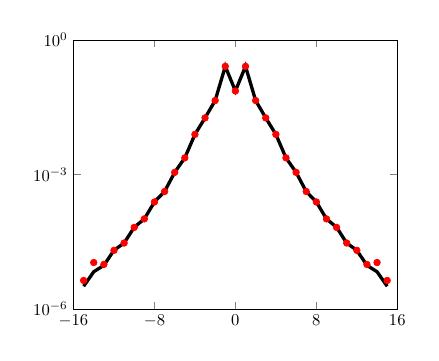
\begin{tikzpicture}[scale=0.6]

\begin{axis}[
  xmin = -16,
  xmax = 16,
  xtick = {-16,-8,0,8,16},
%  xlabel = {Number of Time Steps},
  ymin = 1.0e-6,
  ymax = 1.0e-0,
  ytick = {1e-6,1e-3,1e0},
%  yticklabels = {$10^{-4}$,$10^{-3}$,$10^{-2}$,$10^{-1}$},
  ymode = log,
%  ylabel = {Error},
%  ylabel style = {yshift = 10pt},
%  legend style = {font=\small},
%  legend entries = {no fixes ($N=64$,fix area and length,reduce aliasing,both},
%  legend style = {draw=none},
  ]

% "Exact" single-layer potential
\addplot [color=black,solid,line width=2] table{
-1.5000e+01 3.2060e-06
-1.4000e+01 6.7680e-06
-1.3000e+01 9.3935e-06
-1.2000e+01 2.0365e-05
-1.1000e+01 2.9491e-05
-1.0000e+01 6.6351e-05
-9.0000e+00 1.0226e-04
-8.0000e+00 2.4358e-04
-7.0000e+00 4.1677e-04
-6.0000e+00 1.1132e-03
-5.0000e+00 2.3480e-03
-4.0000e+00 7.8248e-03
-3.0000e+00 1.8265e-02
-2.0000e+00 4.4583e-02
-1.0000e+00 2.5781e-01
0.0000e+00 7.2810e-02
1.0000e+00 2.5781e-01
2.0000e+00 4.4583e-02
3.0000e+00 1.8265e-02
4.0000e+00 7.8248e-03
5.0000e+00 2.3480e-03
6.0000e+00 1.1132e-03
7.0000e+00 4.1677e-04
8.0000e+00 2.4358e-04
9.0000e+00 1.0226e-04
1.0000e+01 6.6351e-05
1.1000e+01 2.9491e-05
1.2000e+01 2.0365e-05
1.3000e+01 9.3935e-06
1.4000e+01 6.7680e-06
1.5000e+01 3.2060e-06
};

% No anti-aliasing; Yes shape correct
\addplot [color=red,only marks,mark=*] table{
-1.5000e+01 4.3190e-06
-1.4000e+01 1.0857e-05
-1.3000e+01 9.8494e-06
-1.2000e+01 2.0313e-05
-1.1000e+01 2.9618e-05
-1.0000e+01 6.5979e-05
-9.0000e+00 1.0227e-04
-8.0000e+00 2.4334e-04
-7.0000e+00 4.1679e-04
-6.0000e+00 1.1131e-03
-5.0000e+00 2.3481e-03
-4.0000e+00 7.8247e-03
-3.0000e+00 1.8265e-02
-2.0000e+00 4.4583e-02
-1.0000e+00 2.5781e-01
0.0000e+00 7.2810e-02
1.0000e+00 2.5781e-01
2.0000e+00 4.4583e-02
3.0000e+00 1.8265e-02
4.0000e+00 7.8247e-03
5.0000e+00 2.3481e-03
6.0000e+00 1.1131e-03
7.0000e+00 4.1679e-04
8.0000e+00 2.4334e-04
9.0000e+00 1.0227e-04
1.0000e+01 6.5979e-05
1.1000e+01 2.9618e-05
1.2000e+01 2.0313e-05
1.3000e+01 9.8494e-06
1.4000e+01 1.0857e-05
1.5000e+01 4.3190e-06
};


\end{axis}


\end{tikzpicture}

 \\
  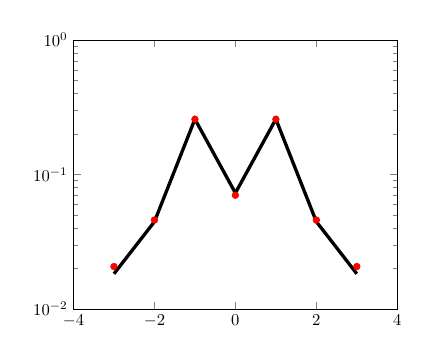
\begin{tikzpicture}[scale=0.6]

\begin{axis}[
  xmin = -4,
  xmax = 4,
  xtick = {-4,-2,0,2,4},
%  xlabel = {Number of Time Steps},
  ymin = 1.0e-2,
  ymax = 1.0e-0,
  ytick = {1e-2,1e-1,1e0},
%  yticklabels = {$10^{-4}$,$10^{-3}$,$10^{-2}$,$10^{-1}$},
  ymode = log,
%  ylabel = {Error},
%  ylabel style = {yshift = 10pt},
%  legend style = {font=\small},
%  legend entries = {no fixes ($N=64$,fix area and length,reduce aliasing,both},
%  legend style = {draw=none},
  ]

% "Exact" single-layer potential
\addplot [color=black,solid,line width=2] table{
-3.0000e+00 1.8265e-02
-2.0000e+00 4.4583e-02
-1.0000e+00 2.5781e-01
0.0000e+00 7.2810e-02
1.0000e+00 2.5781e-01
2.0000e+00 4.4583e-02
3.0000e+00 1.8265e-02
};

% Anti-aliasing with injection
\addplot [color=red,only marks,mark=*] table{
-3.0000e+00 2.0677e-02
-2.0000e+00 4.5861e-02
-1.0000e+00 2.5716e-01
0.0000e+00 7.0125e-02
1.0000e+00 2.5716e-01
2.0000e+00 4.5861e-02
3.0000e+00 2.0677e-02
};


\end{axis}


\end{tikzpicture}

 &
  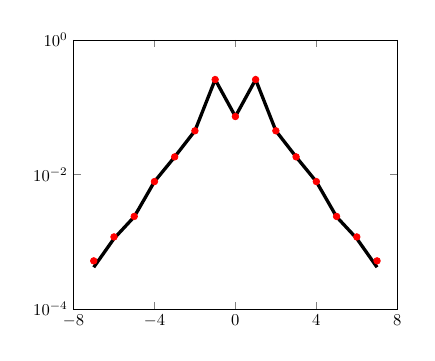
\begin{tikzpicture}[scale=0.6]

\begin{axis}[
  xmin = -8,
  xmax = 8,
  xtick = {-8,-4,0,4,8},
%  xlabel = {Number of Time Steps},
  ymin = 1.0e-4,
  ymax = 1.0e-0,
  ytick = {1e-4,1e-2,1e0},
%  ytick = {1e-4,1e-3,1e-2,1e-1},
%  yticklabels = {$10^{-4}$,$10^{-3}$,$10^{-2}$,$10^{-1}$},
  ymode = log,
%  ylabel = {Error},
%  ylabel style = {yshift = 10pt},
%  legend style = {font=\small},
%  legend entries = {no fixes ($N=64$,fix area and length,reduce aliasing,both},
%  legend style = {draw=none},
  ]

% "Exact" single-layer potential
\addplot [color=black,solid,line width=2] table{
-7.0000e+00 4.1677e-04
-6.0000e+00 1.1132e-03
-5.0000e+00 2.3480e-03
-4.0000e+00 7.8248e-03
-3.0000e+00 1.8265e-02
-2.0000e+00 4.4583e-02
-1.0000e+00 2.5781e-01
0.0000e+00 7.2810e-02
1.0000e+00 2.5781e-01
2.0000e+00 4.4583e-02
3.0000e+00 1.8265e-02
4.0000e+00 7.8248e-03
5.0000e+00 2.3480e-03
6.0000e+00 1.1132e-03
7.0000e+00 4.1677e-04
};

% Anti-aliasing with injection
\addplot [color=red,only marks,mark=*] table{
-7.0000e+00 5.1905e-04
-6.0000e+00 1.1785e-03
-5.0000e+00 2.3777e-03
-4.0000e+00 7.8447e-03
-3.0000e+00 1.8275e-02
-2.0000e+00 4.4594e-02
-1.0000e+00 2.5780e-01
0.0000e+00 7.2771e-02
1.0000e+00 2.5780e-01
2.0000e+00 4.4594e-02
3.0000e+00 1.8275e-02
4.0000e+00 7.8447e-03
5.0000e+00 2.3777e-03
6.0000e+00 1.1785e-03
7.0000e+00 5.1905e-04
};


\end{axis}


\end{tikzpicture}

 &
  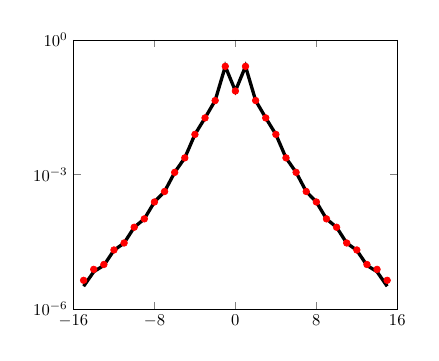
\begin{tikzpicture}[scale=0.6]

\begin{axis}[
  xmin = -16,
  xmax = 16,
  xtick = {-16,-8,0,8,16},
%  xlabel = {Number of Time Steps},
  ymin = 1.0e-6,
  ymax = 1.0e-0,
  ytick = {1e-6,1e-3,1e0},
%  yticklabels = {$10^{-4}$,$10^{-3}$,$10^{-2}$,$10^{-1}$},
  ymode = log,
%  ylabel = {Error},
%  ylabel style = {yshift = 10pt},
%  legend style = {font=\small},
%  legend entries = {no fixes ($N=64$,fix area and length,reduce aliasing,both},
%  legend style = {draw=none},
  ]

% "Exact" single-layer potential
\addplot [color=black,solid,line width=2] table{
-1.5000e+01 3.2060e-06
-1.4000e+01 6.7680e-06
-1.3000e+01 9.3935e-06
-1.2000e+01 2.0365e-05
-1.1000e+01 2.9491e-05
-1.0000e+01 6.6351e-05
-9.0000e+00 1.0226e-04
-8.0000e+00 2.4358e-04
-7.0000e+00 4.1677e-04
-6.0000e+00 1.1132e-03
-5.0000e+00 2.3480e-03
-4.0000e+00 7.8248e-03
-3.0000e+00 1.8265e-02
-2.0000e+00 4.4583e-02
-1.0000e+00 2.5781e-01
0.0000e+00 7.2810e-02
1.0000e+00 2.5781e-01
2.0000e+00 4.4583e-02
3.0000e+00 1.8265e-02
4.0000e+00 7.8248e-03
5.0000e+00 2.3480e-03
6.0000e+00 1.1132e-03
7.0000e+00 4.1677e-04
8.0000e+00 2.4358e-04
9.0000e+00 1.0226e-04
1.0000e+01 6.6351e-05
1.1000e+01 2.9491e-05
1.2000e+01 2.0365e-05
1.3000e+01 9.3935e-06
1.4000e+01 6.7680e-06
1.5000e+01 3.2060e-06
};

% Anti-aliasing with injection
\addplot [color=red,only marks,mark=*] table{
-1.5000e+01 4.3530e-06
-1.4000e+01 7.6387e-06
-1.3000e+01 9.8203e-06
-1.2000e+01 2.0695e-05
-1.1000e+01 2.9656e-05
-1.0000e+01 6.6482e-05
-9.0000e+00 1.0233e-04
-8.0000e+00 2.4363e-04
-7.0000e+00 4.1680e-04
-6.0000e+00 1.1132e-03
-5.0000e+00 2.3480e-03
-4.0000e+00 7.8248e-03
-3.0000e+00 1.8265e-02
-2.0000e+00 4.4583e-02
-1.0000e+00 2.5781e-01
0.0000e+00 7.2810e-02
1.0000e+00 2.5781e-01
2.0000e+00 4.4583e-02
3.0000e+00 1.8265e-02
4.0000e+00 7.8248e-03
5.0000e+00 2.3480e-03
6.0000e+00 1.1132e-03
7.0000e+00 4.1680e-04
8.0000e+00 2.4363e-04
9.0000e+00 1.0233e-04
1.0000e+01 6.6482e-05
1.1000e+01 2.9656e-05
1.2000e+01 2.0695e-05
1.3000e+01 9.8203e-06
1.4000e+01 7.6387e-06
1.5000e+01 4.3530e-06
};


\end{axis}


\end{tikzpicture}

 \\
  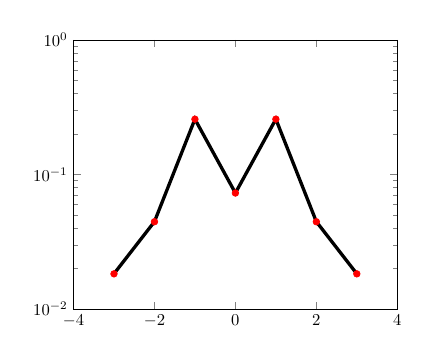
\begin{tikzpicture}[scale=0.6]

\begin{axis}[
  xmin = -4,
  xmax = 4,
  xtick = {-4,-2,0,2,4},
%  xlabel = {Number of Time Steps},
  ymin = 1.0e-2,
  ymax = 1.0e-0,
  ytick = {1e-2,1e-1,1e0},
%  yticklabels = {$10^{-4}$,$10^{-3}$,$10^{-2}$,$10^{-1}$},
  ymode = log,
%  ylabel = {Error},
%  ylabel style = {yshift = 10pt},
%  legend style = {font=\small},
%  legend entries = {no fixes ($N=64$,fix area and length,reduce aliasing,both},
%  legend style = {draw=none},
  ]

% "Exact" single-layer potential
\addplot [color=black,solid,line width=2] table{
-3.0000e+00 1.8265e-02
-2.0000e+00 4.4583e-02
-1.0000e+00 2.5781e-01
0.0000e+00 7.2810e-02
1.0000e+00 2.5781e-01
2.0000e+00 4.4583e-02
3.0000e+00 1.8265e-02
};

% Anti-aliasing with spectral restriction
\addplot [color=red,only marks,mark=*] table{
-3.0000e+00 1.8246e-02
-2.0000e+00 4.4515e-02
-1.0000e+00 2.5768e-01
0.0000e+00 7.2780e-02
1.0000e+00 2.5768e-01
2.0000e+00 4.4515e-02
3.0000e+00 1.8246e-02
};


\end{axis}


\end{tikzpicture}

 &
  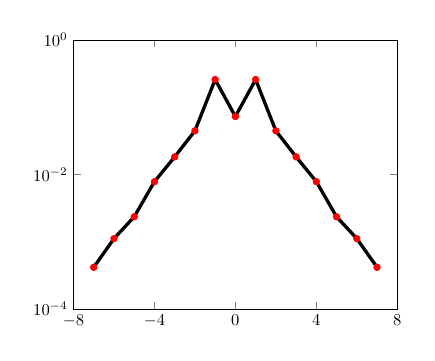
\begin{tikzpicture}[scale=0.6]

\begin{axis}[
  xmin = -8,
  xmax = 8,
  xtick = {-8,-4,0,4,8},
%  xlabel = {Number of Time Steps},
  ymin = 1.0e-4,
  ymax = 1.0e-0,
  ytick = {1e-4,1e-2,1e0},
%  ytick = {1e-4,1e-3,1e-2,1e-1},
%  yticklabels = {$10^{-4}$,$10^{-3}$,$10^{-2}$,$10^{-1}$},
  ymode = log,
%  ylabel = {Error},
%  ylabel style = {yshift = 10pt},
%  legend style = {font=\small},
%  legend entries = {no fixes ($N=64$,fix area and length,reduce aliasing,both},
%  legend style = {draw=none},
  ]

% "Exact" single-layer potential
\addplot [color=black,solid,line width=2] table{
-7.0000e+00 4.1677e-04
-6.0000e+00 1.1132e-03
-5.0000e+00 2.3480e-03
-4.0000e+00 7.8248e-03
-3.0000e+00 1.8265e-02
-2.0000e+00 4.4583e-02
-1.0000e+00 2.5781e-01
0.0000e+00 7.2810e-02
1.0000e+00 2.5781e-01
2.0000e+00 4.4583e-02
3.0000e+00 1.8265e-02
4.0000e+00 7.8248e-03
5.0000e+00 2.3480e-03
6.0000e+00 1.1132e-03
7.0000e+00 4.1677e-04
};

% Anti-aliasing with spectral restriction
\addplot [color=red,only marks,mark=*] table{
-7.0000e+00 4.1678e-04
-6.0000e+00 1.1131e-03
-5.0000e+00 2.3481e-03
-4.0000e+00 7.8247e-03
-3.0000e+00 1.8265e-02
-2.0000e+00 4.4583e-02
-1.0000e+00 2.5781e-01
0.0000e+00 7.2810e-02
1.0000e+00 2.5781e-01
2.0000e+00 4.4583e-02
3.0000e+00 1.8265e-02
4.0000e+00 7.8247e-03
5.0000e+00 2.3481e-03
6.0000e+00 1.1131e-03
7.0000e+00 4.1678e-04
};


\end{axis}


\end{tikzpicture}

 &
  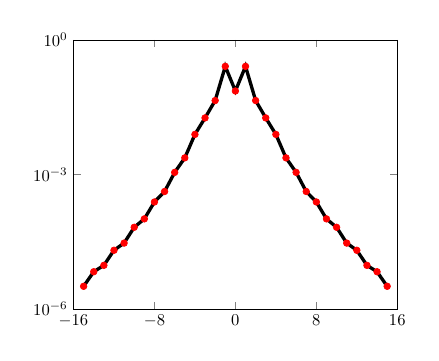
\begin{tikzpicture}[scale=0.6]

\begin{axis}[
  xmin = -16,
  xmax = 16,
  xtick = {-16,-8,0,8,16},
%  xlabel = {Number of Time Steps},
  ymin = 1.0e-6,
  ymax = 1.0e-0,
  ytick = {1e-6,1e-3,1e0},
%  yticklabels = {$10^{-4}$,$10^{-3}$,$10^{-2}$,$10^{-1}$},
  ymode = log,
%  ylabel = {Error},
%  ylabel style = {yshift = 10pt},
%  legend style = {font=\small},
%  legend entries = {no fixes ($N=64$,fix area and length,reduce aliasing,both},
%  legend style = {draw=none},
  ]

% "Exact" single-layer potential
\addplot [color=black,solid,line width=2] table{
-1.5000e+01 3.2060e-06
-1.4000e+01 6.7680e-06
-1.3000e+01 9.3935e-06
-1.2000e+01 2.0365e-05
-1.1000e+01 2.9491e-05
-1.0000e+01 6.6351e-05
-9.0000e+00 1.0226e-04
-8.0000e+00 2.4358e-04
-7.0000e+00 4.1677e-04
-6.0000e+00 1.1132e-03
-5.0000e+00 2.3480e-03
-4.0000e+00 7.8248e-03
-3.0000e+00 1.8265e-02
-2.0000e+00 4.4583e-02
-1.0000e+00 2.5781e-01
0.0000e+00 7.2810e-02
1.0000e+00 2.5781e-01
2.0000e+00 4.4583e-02
3.0000e+00 1.8265e-02
4.0000e+00 7.8248e-03
5.0000e+00 2.3480e-03
6.0000e+00 1.1132e-03
7.0000e+00 4.1677e-04
8.0000e+00 2.4358e-04
9.0000e+00 1.0226e-04
1.0000e+01 6.6351e-05
1.1000e+01 2.9491e-05
1.2000e+01 2.0365e-05
1.3000e+01 9.3935e-06
1.4000e+01 6.7680e-06
1.5000e+01 3.2060e-06
};

% Anti-aliasing with spectral restriction
\addplot [color=red,only marks,mark=*] table{
-1.5000e+01 3.2039e-06
-1.4000e+01 6.7657e-06
-1.3000e+01 9.3923e-06
-1.2000e+01 2.0364e-05
-1.1000e+01 2.9492e-05
-1.0000e+01 6.6353e-05
-9.0000e+00 1.0227e-04
-8.0000e+00 2.4358e-04
-7.0000e+00 4.1678e-04
-6.0000e+00 1.1132e-03
-5.0000e+00 2.3480e-03
-4.0000e+00 7.8248e-03
-3.0000e+00 1.8265e-02
-2.0000e+00 4.4583e-02
-1.0000e+00 2.5781e-01
0.0000e+00 7.2810e-02
1.0000e+00 2.5781e-01
2.0000e+00 4.4583e-02
3.0000e+00 1.8265e-02
4.0000e+00 7.8248e-03
5.0000e+00 2.3480e-03
6.0000e+00 1.1132e-03
7.0000e+00 4.1678e-04
8.0000e+00 2.4358e-04
9.0000e+00 1.0227e-04
1.0000e+01 6.6353e-05
1.1000e+01 2.9492e-05
1.2000e+01 2.0364e-05
1.3000e+01 9.3923e-06
1.4000e+01 6.7657e-06
1.5000e+01 3.2039e-06
};


\end{axis}


\end{tikzpicture}


  \end{tabular}
  \mcaption{(Top: The spectrum of the exact single-layer potential
  (black line) and the approximate layer potentials using $N=8, 16, 32$
  points (red circles) for an elliptical geometry.  Middle: The spectrum
  of the exact single-layer potential (black line) and the approximate
  layer potentials at $N=8, 16, 32$ points (red circles) for an
  elliptical geometry.  The aliasing error is reduced since the
  quadrature rule is applied to $2N$, rather than $N$, source points.
  Bottom: The spectrum of the exact single-layer potential (black line)
  and the approximate layer potentials at $N=8, 16, 32$ points (red
  circles) for an elliptical geometry.  The aliasing error is further
  reduced since the quadrature rule is applied to $2N$, rather than $N$,
  source and target points.  Then, the layer potential is restricted to
  $N$ points using Fourier restriction.}{f:aliasingErrors}
\end{figure}

We investigate two strategies to reduce aliasing.  The first method is
to upsample $\gamma$ at some specified rate, and then evaluate the layer
potential at the original $N$ points on the coarse grid, or
equivalently, we restrict with injection.  The required number of
operations, without the FMM, is $\mathcal{O}(\alpha N^{2}),$ where
$\alpha$ is the upsampling rate.  Figure~\ref{f:aliasingErrors} shows a
reduction in the aliasing error, albeit a slight one.  As an
alternative, we test spectral restriction.  We again use Alpert's
quadrature rule on an upsampled grid, but then compute the layer
potential on the upsampled grid.  Then, we use Fourier interpolation to
restrict the layer potential to the coarse grid.  The resulting errors
are in Figure~\ref{f:aliasingErrors}.  Unsurprisingly, the aliasing
errors for spectral restriction are less than those that use injection.
However, there is an additional computational cost as this method
requires $\mathcal{O}(\alpha^{2}N^{2} + \alpha N \log(\alpha N))$
operations.

We summarize the errors of these two strategies in
Tables~\ref{t:ellipseSLPErrors}--\ref{t:flowerSLPErrors} (single-layer
potential) and Tables~\ref{t:ellipseDLPErrors}--\ref{t:flowerDLPErrors}
(double-layer potential).  Since instabilities often occur because of
errors that first occur in the high frequencies, we separately report
the relative errors for the low and high frequencies.  The restriction
is done either with injection or spectrally, and we consider upsampling
by 2 as well as 4.  As expected, the spectral restriction is more
accurate, but it is also more expensive.  Nonetheless, given the values
of $N$ of interest, we can justify this additional cost.  We see that
the double-layer potential is less prone to aliasing, and, also,
upsampling by a factor of 4 does not offer much more accuracy than
upsampling by 2.  Therefore, when evaluating layer potentials, we
upsample by a factor of 2 and use spectral restriction.


\begin{table}[htpb]
\centering
\begin{tabular}{c|cc|cc|cc|cc|cc|}
 & \multicolumn{2}{c|}{$1 \times$} 
 & \multicolumn{2}{c|}{$2 \times$ \: injection}
 & \multicolumn{2}{c|}{$4 \times$ \: injection}
 & \multicolumn{2}{c|}{$2 \times$ \: spectral}
 & \multicolumn{2}{c|}{$4 \times$ \: spectral} \\
 $N$ & Low & High & Low & High & Low & High & Low & High & Low & High \\
 \hline
 8  & 8.88e-3 & 2.38e-2
    & 2.84e-3 & 3.93e-3
    & 9.44e-4 & 3.76e-3
    & 1.80e-4 & 2.37e-4
    & 4.98e-5 & 1.81e-4
    \\
 12 & 1.55e-3 & 4.48e-3
    & 3.25e-4 & 7.03e-4
    & 1.25e-4 & 7.03e-4
    & 4.88e-6 & 6.35e-6
    & 1.61e-6 & 2.28e-6
    \\
 16 & 1.63e-4 & 1.04e-3
    & 4.45e-5 & 1.79e-4
    & 1.93e-5 & 1.80e-4
    & 1.88e-7 & 1.66e-7 
    & 1.34e-8 & 3.71e-8
    \\
 24 & 6.27e-6 & 8.78e-5
    & 1.37e-6 & 1.74e-5
    & 8.68e-7 & 1.74e-5
    & 5.42e-8 & 1.06e-7
    & 4.58e-9 & 6.76e-9
    \\
 32 & 2.57e-7 & 1.04e-5
    & 8.58e-8 & 2.20e-6
    & 5.46e-8 & 2.21e-6
    & 3.02e-8 & 3.66e-8
    & 1.88e-9 & 1.82e-9
\end{tabular}
\mcaption{The errors for approximating the single-layer potential for
the elliptical geometry.}{t:ellipseSLPErrors}

\begin{tabular}{c|cc|cc|cc|cc|cc|}
 & \multicolumn{2}{c|}{$1 \times$} 
 & \multicolumn{2}{c|}{$2 \times$ \: injection}
 & \multicolumn{2}{c|}{$4 \times$ \: injection}
 & \multicolumn{2}{c|}{$2 \times$ \: spectral}
 & \multicolumn{2}{c|}{$4 \times$ \: spectral} \\
 $N$ & Low & High & Low & High & Low & High & Low & High & Low & High \\
 \hline
 8  & 4.32e-2 & 5.02e-2
    & 3.93e-2 & 2.94e-2
    & 3.62e-2 & 2.92e-2
    & 3.57e-2 & 2.84e-2
    & 3.54e-2 & 2.80e-2
    \\
 12 & 4.98e-2 & 1.17e-2
    & 4.55e-2 & 1.36e-2
    & 4.39e-2 & 1.40e-2
    & 4.38e-2 & 1.34e-2
    & 4.36e-2 & 1.34e-2
    \\
 16 & 4.50e-2 & 1.61e-2
    & 4.39e-2 & 1.53e-2
    & 4.37e-2 & 1.53e-2
    & 4.37e-2 & 1.52e-2
    & 4.37e-2 & 1.52e-2
    \\
 24 & 3.55e-2 & 3.44e-2
    & 2.46e-2 & 1.97e-2
    & 2.30e-2 & 1.91e-2
    & 3.02e-2 & 1.96e-2
    & 2.47e-2 & 1.79e-2
    \\
 32 & 1.11e-2 & 4.54e-3
    & 1.67e-3 & 1.78e-3
    & 4.29e-4 & 1.83e-3
    & 4.55e-4 & 5.04e-5
    & 4.21e-5 & 2.83e-5
    \\
 48 & 1.83e-3 & 2.69e-3
    & 1.65e-4 & 4.25e-4
    & 4.77e-5 & 4.31e-4
    & 3.54e-5 & 7.75e-6
    & 1.65e-6 & 1.06e-6
\end{tabular}
\mcaption{The errors for approximating the single-layer potential for
the curly geometry.}{t:curlySLPErrors}

\begin{tabular}{c|cc|cc|cc|cc|cc|}
 & \multicolumn{2}{c|}{$1 \times$} 
 & \multicolumn{2}{c|}{$2 \times$ \: injection}
 & \multicolumn{2}{c|}{$4 \times$ \: injection}
 & \multicolumn{2}{c|}{$2 \times$ \: spectral}
 & \multicolumn{2}{c|}{$4 \times$ \: spectral} \\
 $N$ & Low & High & Low & High & Low & High & Low & High & Low & High \\
 \hline
 8  & 3.61e-2 & 9.64e-2
    & 5.74e-2 & 8.20e-2
    & 5.57e-2 & 8.26e-2
    & 5.49e-2 & 7.38e-2
    & 5.51e-2 & 7.38e-2
    \\
 12 & 5.28e-2 & 4.04e-2
    & 2.86e-2 & 3.26e-2
    & 1.09e-2 & 3.34e-2
    & 9.84e-3 & 3.74e-2
    & 7.60e-3 & 3.73e-2
    \\
 16 & 7.83e-3 & 8.19e-3
    & 1.47e-3 & 3.82e-3
    & 6.35e-4 & 3.85e-3
    & 1.44e-4 & 1.30e-4
    & 6.79e-7 & 3.36e-7
    \\
 24 & 8.74e-4 & 1.16e-3
    & 1.96e-4 & 5.84e-4
    & 1.46e-4 & 5.93e-4
    & 4.45e-6 & 6.22e-6
    & 1.24e-8 & 1.23e-7
    \\
 32 & 1.94e-4 & 3.08e-4
    & 2.90e-5 & 2.32e-4
    & 2.63e-5 & 2.32e-4
    & 7.05e-6 & 5.50e-7
    & 6.64e-9 & 4.50e-8
    \\
 48 & 7.64e-6 & 3.78e-5
    & 1.10e-6 & 2.72e-5
    & 1.13e-6 & 2.73e-5
    & 1.24e-7 & 1.10e-7
    & 7.09e-9 & 7.84e-9
\end{tabular}
\mcaption{The errors for approximating the single-layer potential for
the flower geometry.}{t:flowerSLPErrors}
\end{table}

% DOUBLE-LAYER POTENTIAL
\begin{table}[htpb]
\centering
\begin{tabular}{c|cc|cc|cc|cc|cc|}
 & \multicolumn{2}{c|}{$1 \times$} 
 & \multicolumn{2}{c|}{$2 \times$ \: injection}
 & \multicolumn{2}{c|}{$4 \times$ \: injection}
 & \multicolumn{2}{c|}{$2 \times$ \: spectral}
 & \multicolumn{2}{c|}{$4 \times$ \: spectral} \\
 $N$ & Low & High & Low & High & Low & High & Low & High & Low & High \\
 \hline
 8  & 3.07e-2 & 1.25e-2
    & 2.66e-4 & 2.30e-4
    & 1.65e-7 & 3.22e-4
    & 2.66e-4 & 2.30e-4
    & 1.65e-7 & 3.22e-4
    \\
 12 & 3.37e-3 & 3.66e-4
    & 1.67e-6 & 8.16e-6
    & 7.72e-7 & 8.36e-6
    & 1.67e-6 & 8.16e-6
    & 7.72e-7 & 8.36e-6
    \\
 16 & 2.93e-4 & 3.12e-5
    & 9.10e-9 & 1.45e-7
    & 1.24e-9 & 1.46e-7
    & 9.10e-9 & 1.45e-7
    & 1.24e-9 & 1.46e-7
    \\
 24 & 1.80e-6 & 4.47e-8
    & 2.19e-13 & 2.44e-11
    & 2.45e-14 & 2.44e-11
    & 2.20e-13 & 2.44e-11
    & 2.43e-14 & 2.44e-11
    \\
 32 & 9.55e-9 & 4.85e-11
    & 1.09e-15 & 2.45e-15
    & 2.02e-15 & 3.05e-15
    & 1.86e-16 & 2.65e-15
    & 2.49e-16 & 2.36e-15
\end{tabular}
\mcaption{The errors for approximating the double-layer potential for
the elliptical geometry.}{t:ellipseDLPErrors}

\begin{tabular}{c|cc|cc|cc|cc|cc|}
 & \multicolumn{2}{c|}{$1 \times$} 
 & \multicolumn{2}{c|}{$2 \times$ \: injection}
 & \multicolumn{2}{c|}{$4 \times$ \: injection}
 & \multicolumn{2}{c|}{$2 \times$ \: spectral}
 & \multicolumn{2}{c|}{$4 \times$ \: spectral} \\
 $N$ & Low & High & Low & High & Low & High & Low & High & Low & High \\
 \hline
 8  & 1.53e-3 & 2.79e-2
    & 5.46e-3 & 1.97e-2
    & 6.18e-3 & 1.90e-2
    & 5.99e-3 & 1.78e-2
    & 6.17e-3 & 1.75e-2
    \\
 12 & 7.33e-3 & 1.33e-2
    & 3.14e-3 & 6.37e-3
    & 3.07e-3 & 6.27e-3
    & 2.86e-3 & 5.72e-3
    & 2.78e-3 & 5.66e-3
    \\
 16 & 2.13e-2 & 7.81e-3
    & 2.07e-2 & 9.24e-3
    & 2.07e-2 & 9.24e-3
    & 2.07e-2 & 9.01e-3
    & 2.07e-2 & 9.01e-3
    \\
 24 & 7.93e-2 & 1.23e-1
    & 5.44e-1 & 5.75e-1
    & 3.82e-1 & 4.04e-1
    & 4.28e-1 & 3.73e-1
    & 3.55e-1 & 3.10e-1
    \\
 32 & 1.54e-2 & 3.79e-2
    & 2.59e-3 & 2.82e-3
    & 1.78e-4 & 1.62e-3
    & 9.29e-4 & 1.20e-3
    & 6.76e-6 & 1.28e-5
    \\
 48 & 7.05e-3 & 1.32e-2
    & 1.25e-4 & 2.66e-4
    & 1.14e-5 & 1.64e-4
    & 3.55e-5 & 8.67e-5
    & 3.64e-7 & 5.91e-7
\end{tabular}
\mcaption{The errors for approximating the double-layer potential for
the curly geometry.}{t:curlyDLPErrors}

\begin{tabular}{c|cc|cc|cc|cc|cc|}
 & \multicolumn{2}{c|}{$1 \times$} 
 & \multicolumn{2}{c|}{$2 \times$ \: injection}
 & \multicolumn{2}{c|}{$4 \times$ \: injection}
 & \multicolumn{2}{c|}{$2 \times$ \: spectral}
 & \multicolumn{2}{c|}{$4 \times$ \: spectral} \\
 $N$ & Low & High & Low & High & Low & High & Low & High & Low & High \\
 \hline
 8  & 7.86e-2 & 1.40e-1
    & 5.21e-2 & 8.38e-2
    & 5.16e-2 & 8.50e-2
    & 5.19e-2 & 8.29e-2
    & 5.18e-2 & 8.37e-2
    \\
 12 & 1.02e-1 & 1.40e-1
    & 2.84e-2 & 3.45e-2
    & 1.20e-2 & 2.50e-2
    & 2.46e-2 & 3.51e-2
    & 1.21e-2 & 2.62e-2
    \\
 16 & 1.92e-2 & 2.83e-2
    & 6.87e-4 & 3.83e-3
    & 3.09e-4 & 3.77e-3
    & 2.75e-4 & 5.09e-4
    & 4.27e-7 & 4.06e-7
    \\
 24 & 3.60e-3 & 4.99e-3
    & 4.13e-5 & 2.86e-4
    & 3.48e-5 & 2.86e-4
    & 5.63e-6 & 9.52e-6
    & 1.96e-10 & 2.56e-10
    \\
 32 & 5.79e-4 & 7.03e-4
    & 2.88e-6 & 3.94e-5
    & 2.71e-6 & 3.93e-5
    & 9.83e-8 & 2.93e-7
    & 1.31e-13 & 7.80e-13
    \\
 48 & 1.11e-5 & 2.67e-5
    & 9.84e-9 & 2.72e-6
    & 9.77e-9 & 2.72e-6
    & 3.17e-11 & 8.96e-11
    & 4.55e-16 & 5.86e-16
\end{tabular}
\mcaption{The errors for approximating the double-layer potential for
the flower geometry.}{t:flowerDLPErrors}
\end{table}

Another major source of aliasing error comes from computing the traction
jump.  In particular, given a vesicle shape $\xx$ with tension $\sigma$,
we have to compute $\ff = -\xx_{ssss} + (\sigma \xx_{s})_{s}$, where we
have normalized the bending modulus to one.  As before, we test the
effect of aliasing by picking an arbitrary tension $\sigma =
\exp(\cos(\theta))$ and then computing the traction jump $\ff$ on a fine
grid to form a reference solution.  We consider spectral restriction
since we are interested in small values $N$ so that the additional cost
as compared to injection is not significant.  In
Figure~\ref{f:tracAliasingError}
\todo{Draw some conclusions as to the upsampling rate.  I expect that it
should be 4 or maybe even 8.}


\begin{figure}[htpb]
  \centering
  \begin{tabular}{ccc}
  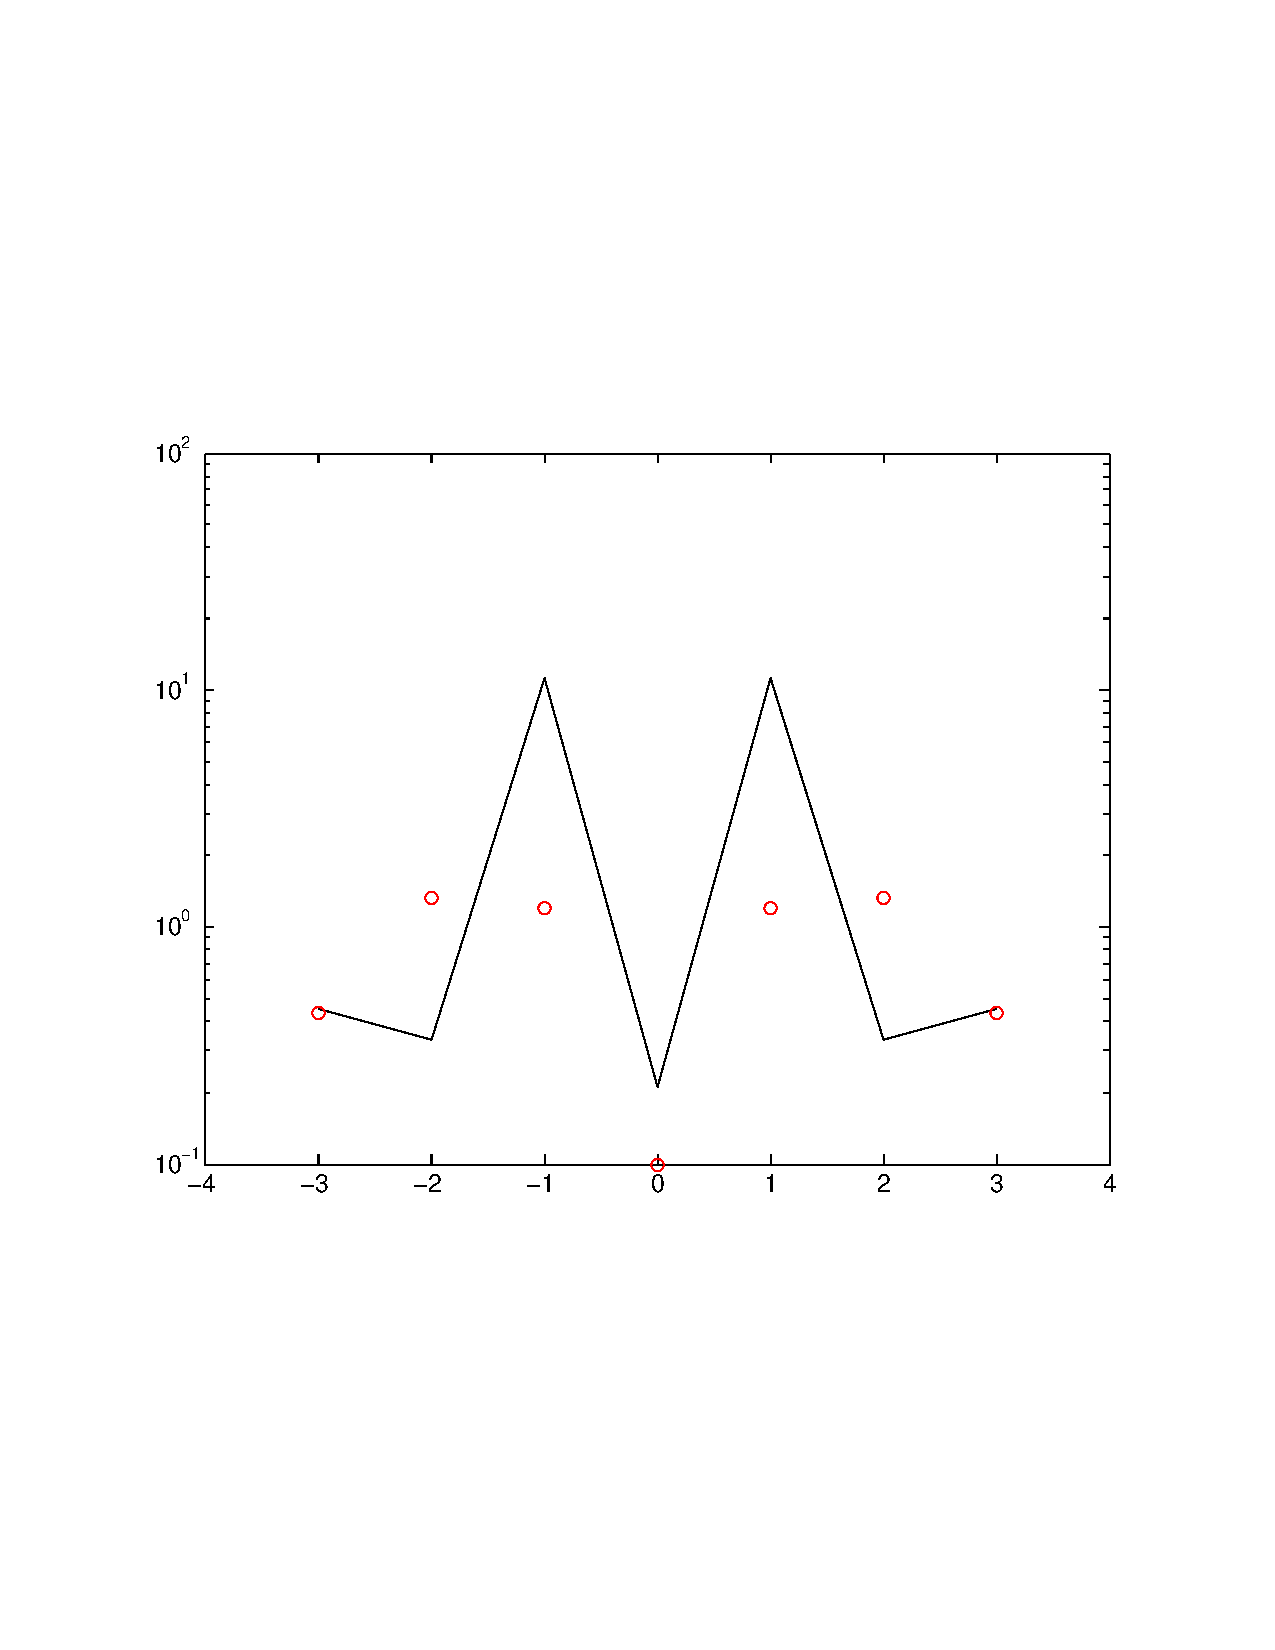
\includegraphics[scale=0.25]{figs/tracAliasingUp1N08} &
  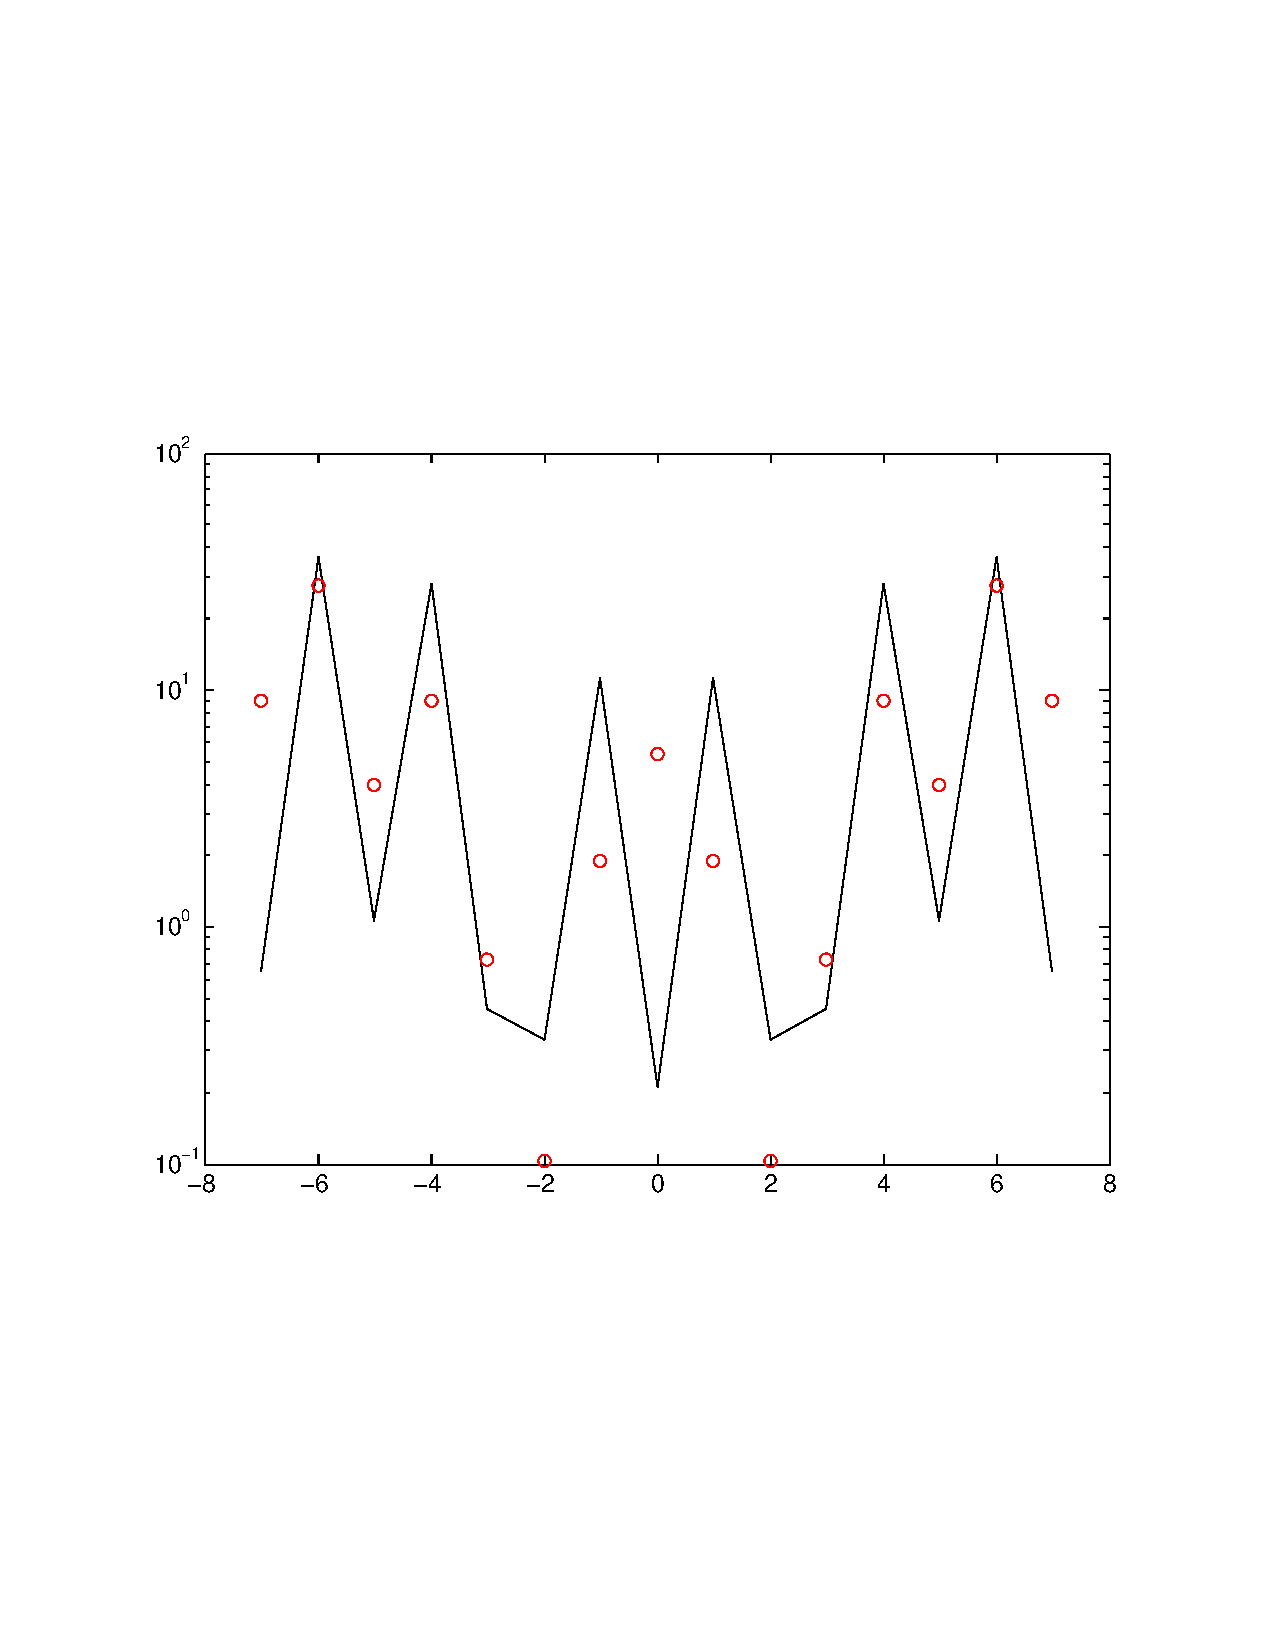
\includegraphics[scale=0.25]{figs/tracAliasingUp1N16} &
  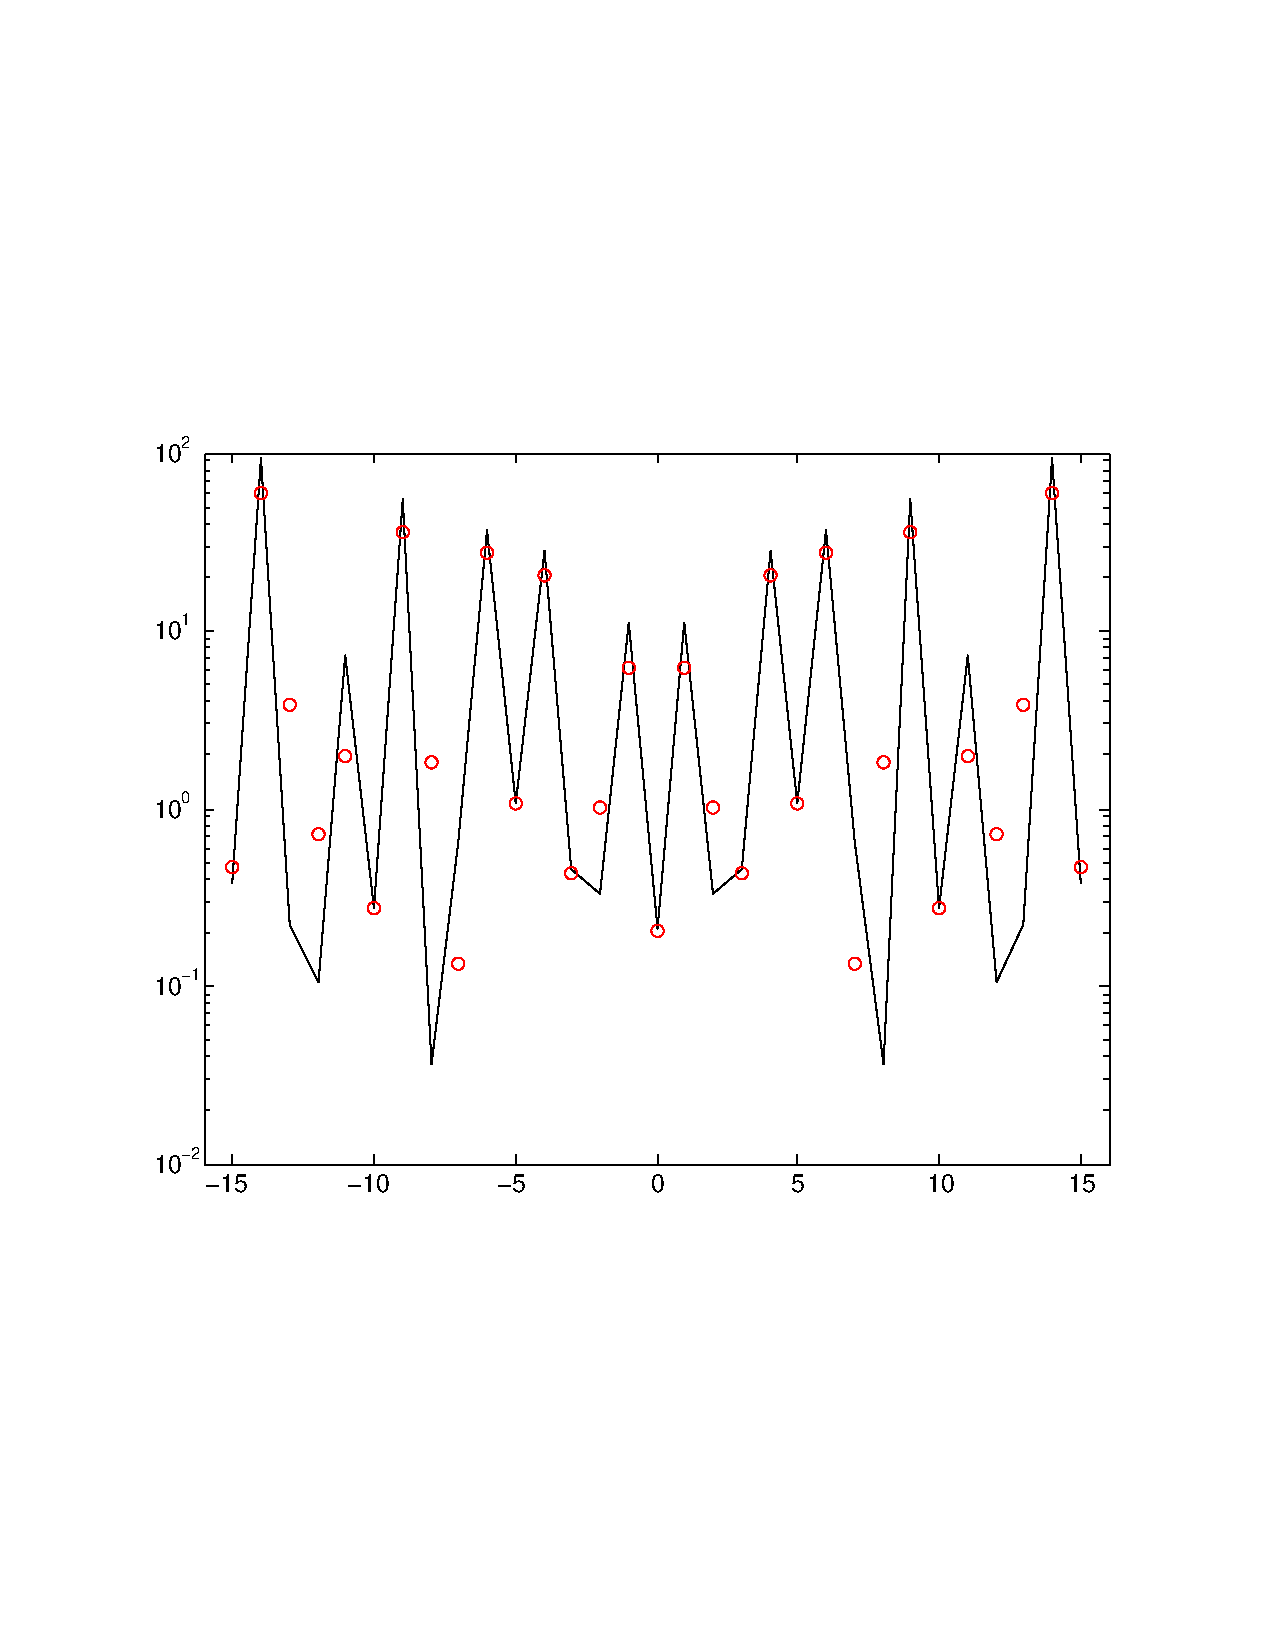
\includegraphics[scale=0.25]{figs/tracAliasingUp1N32} \\
  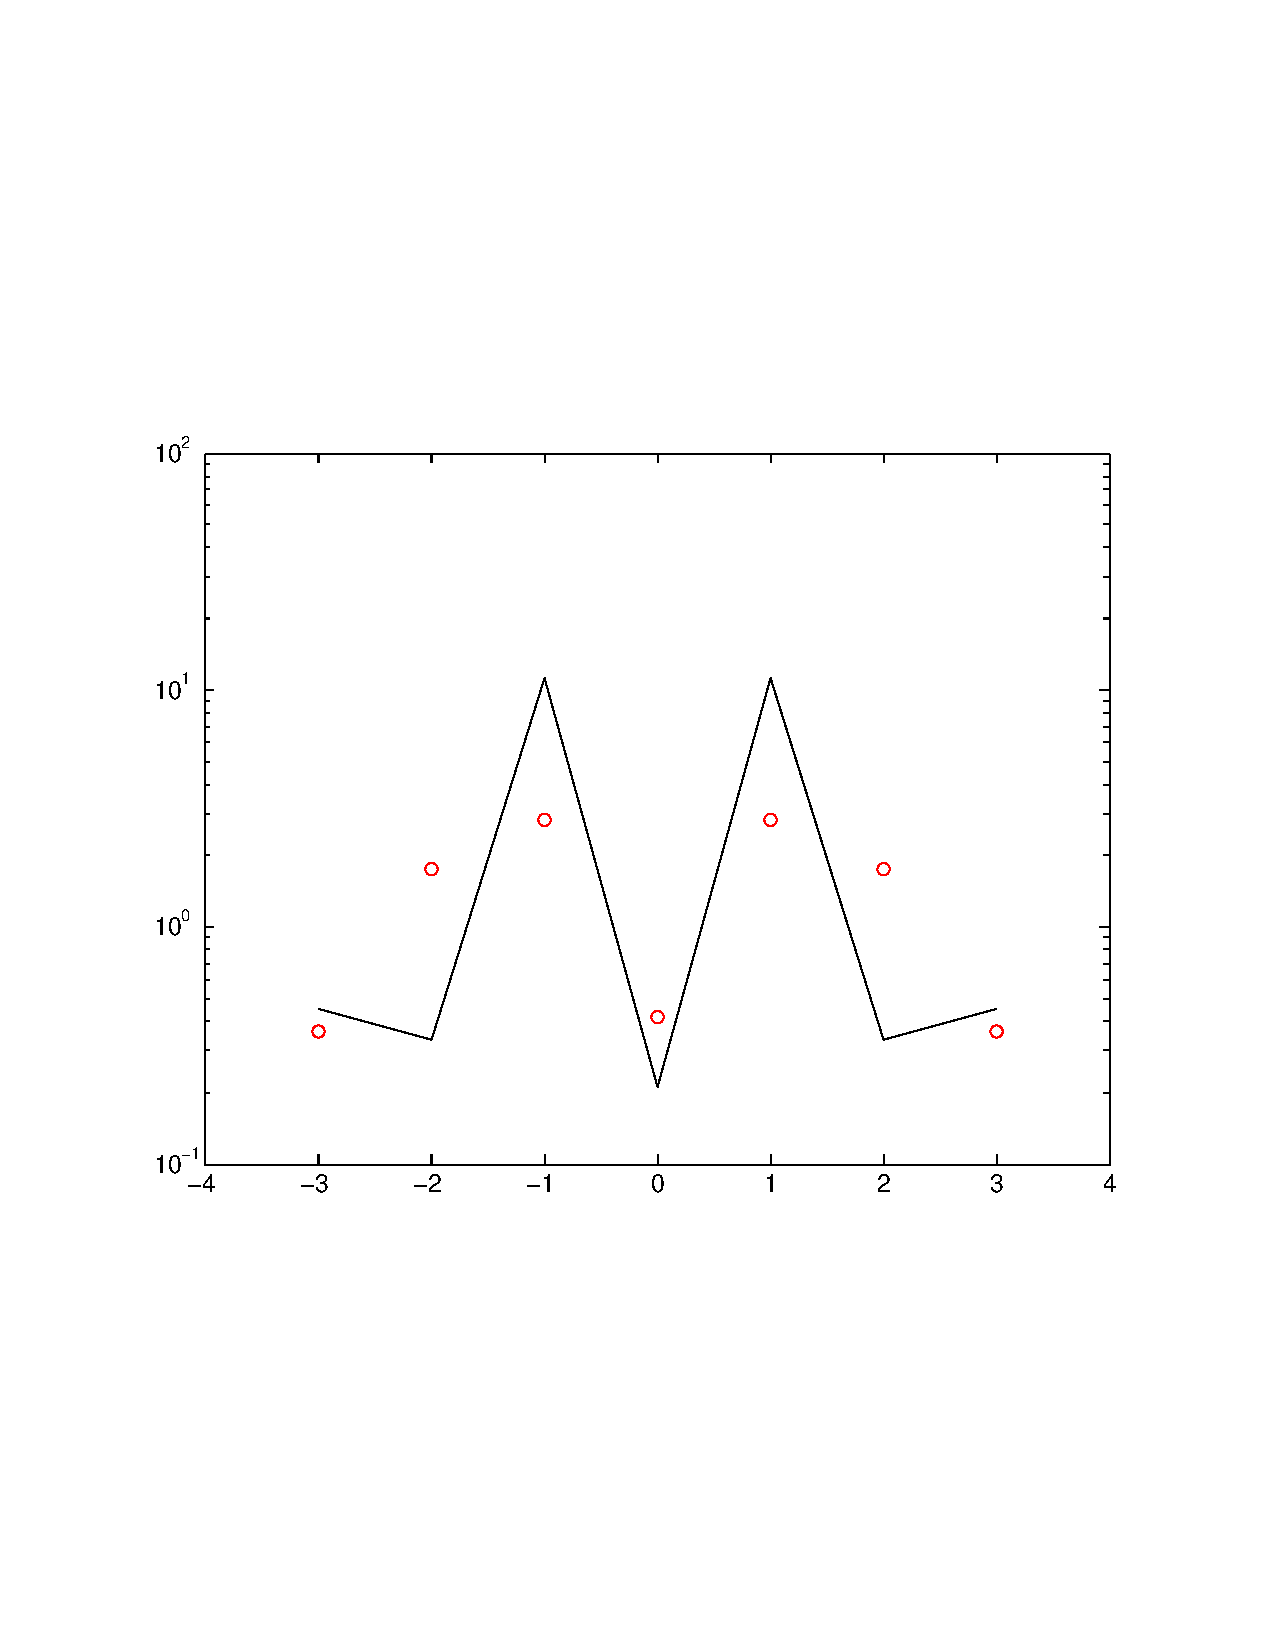
\includegraphics[scale=0.25]{figs/tracAliasingUp2N08} &
  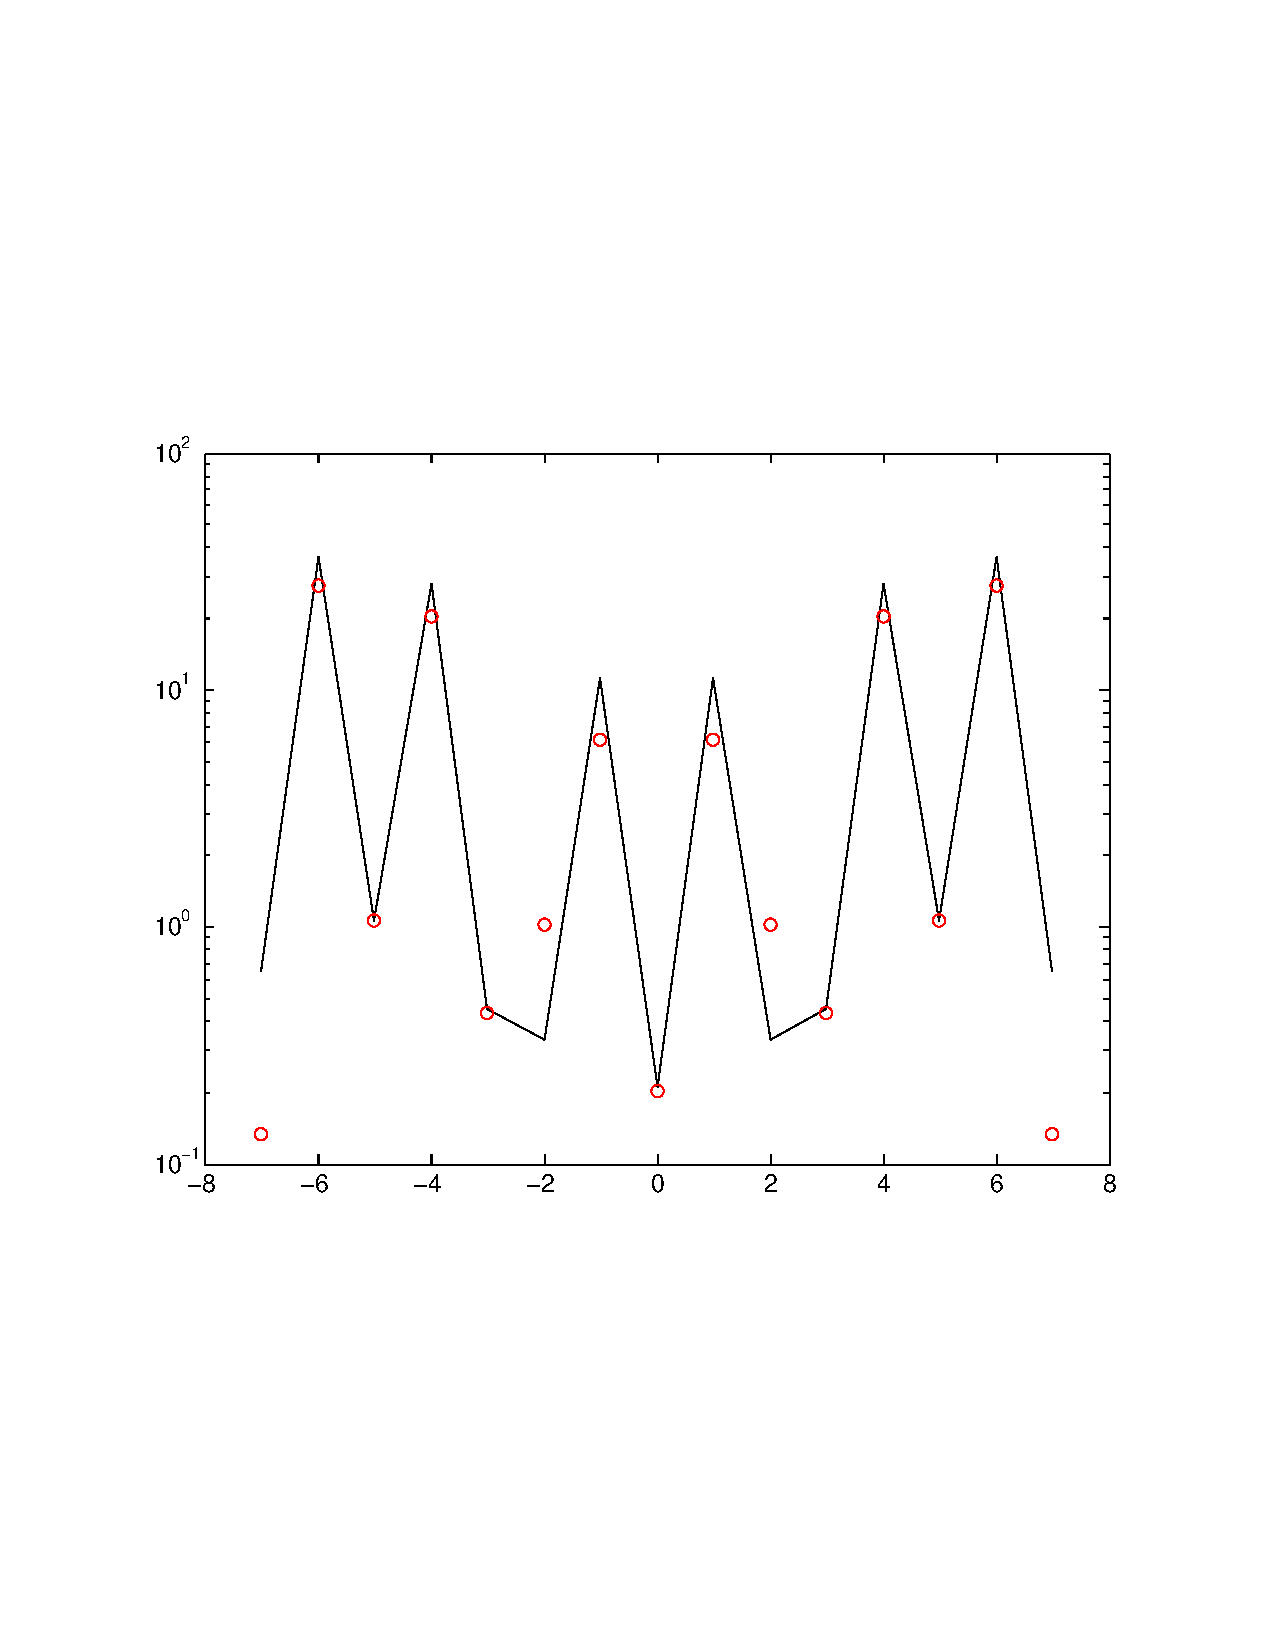
\includegraphics[scale=0.25]{figs/tracAliasingUp2N16} &
  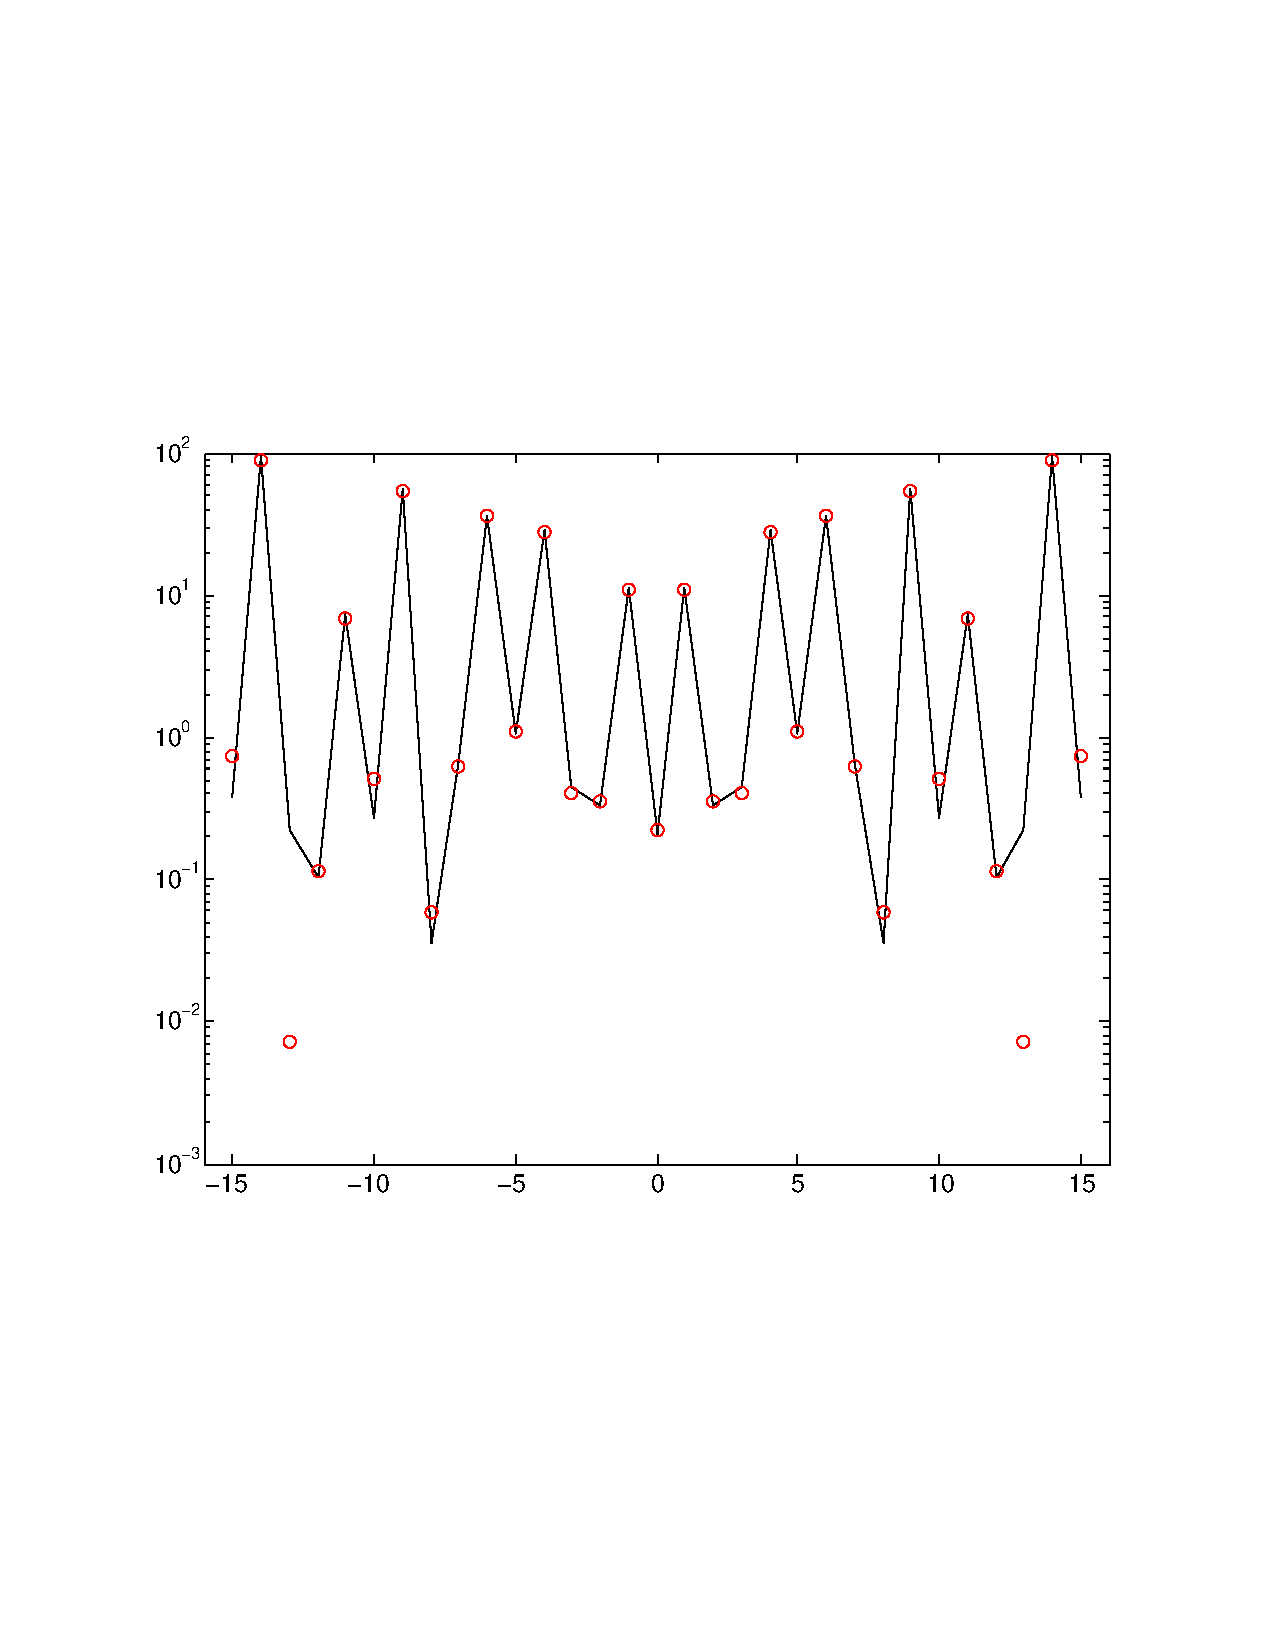
\includegraphics[scale=0.25]{figs/tracAliasingUp2N32} \\
  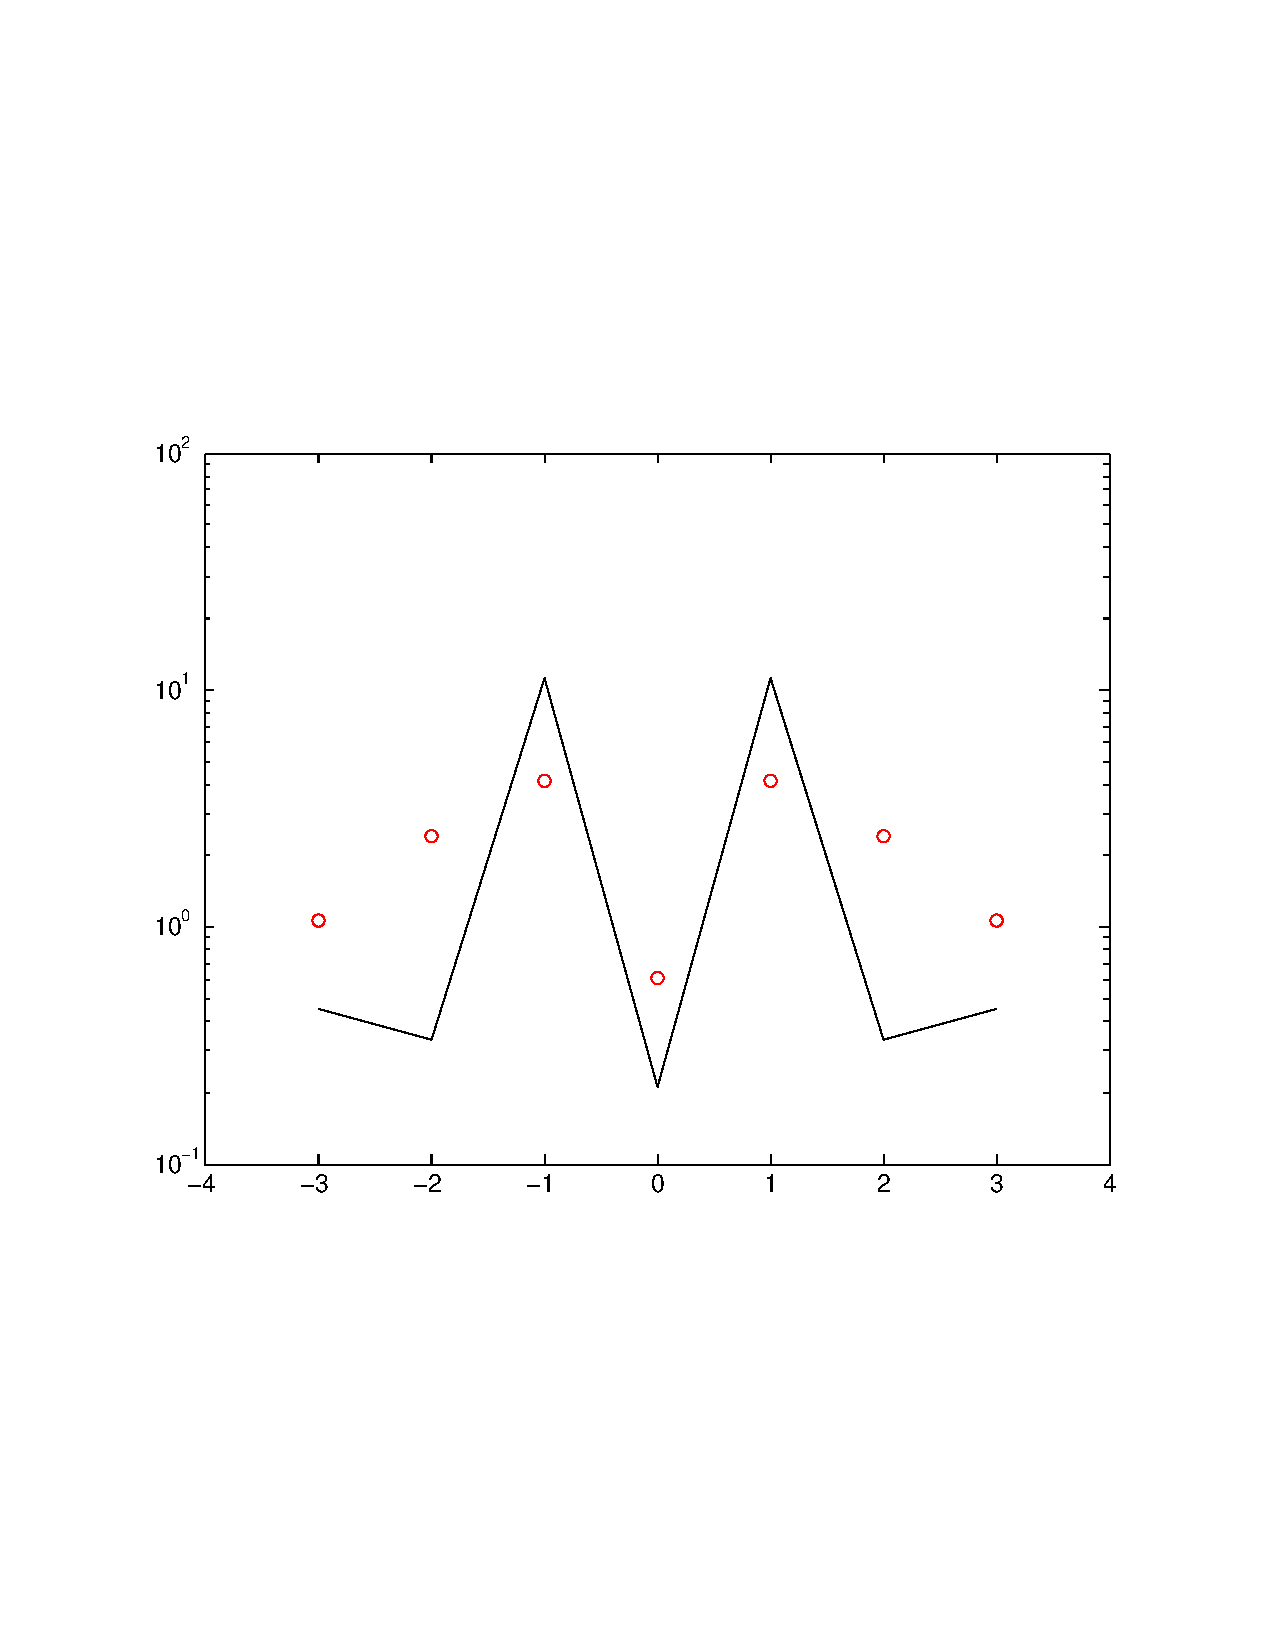
\includegraphics[scale=0.25]{figs/tracAliasingUp4N08} &
  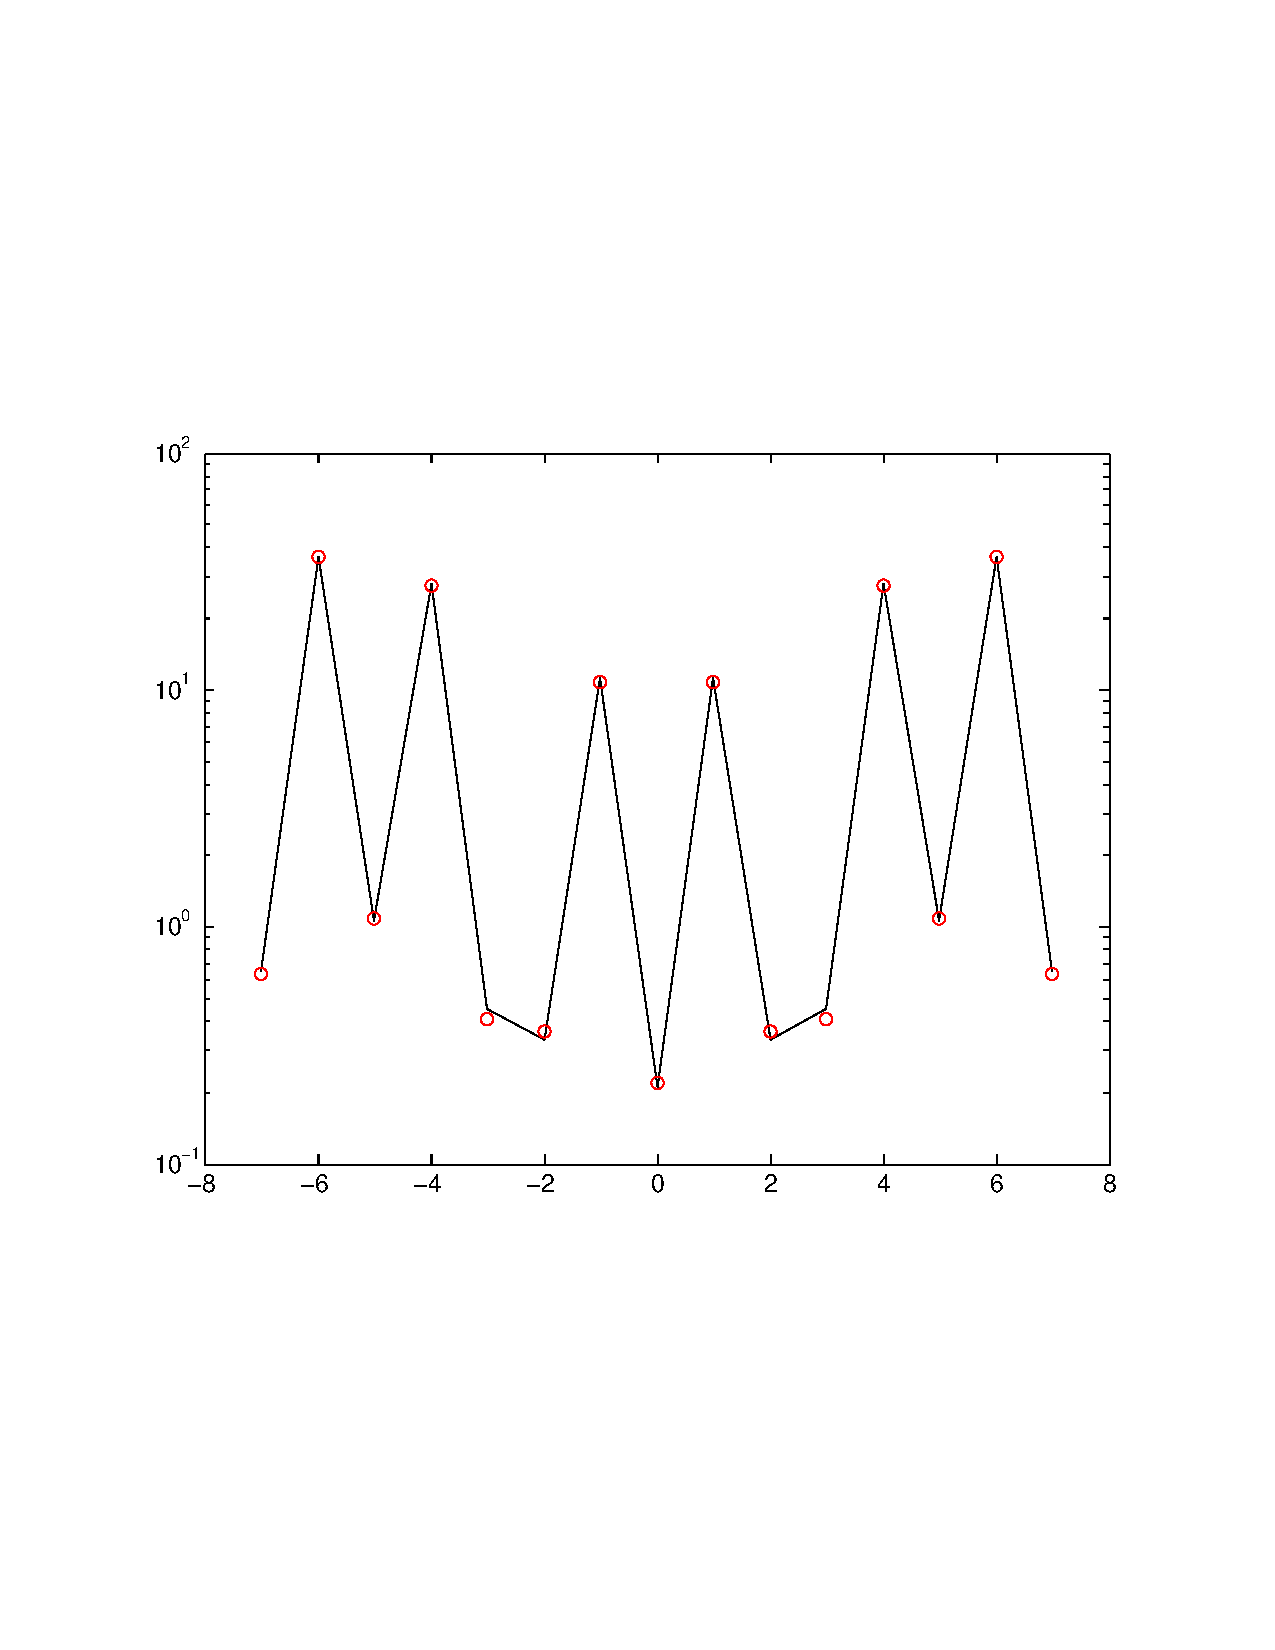
\includegraphics[scale=0.25]{figs/tracAliasingUp4N16} &
  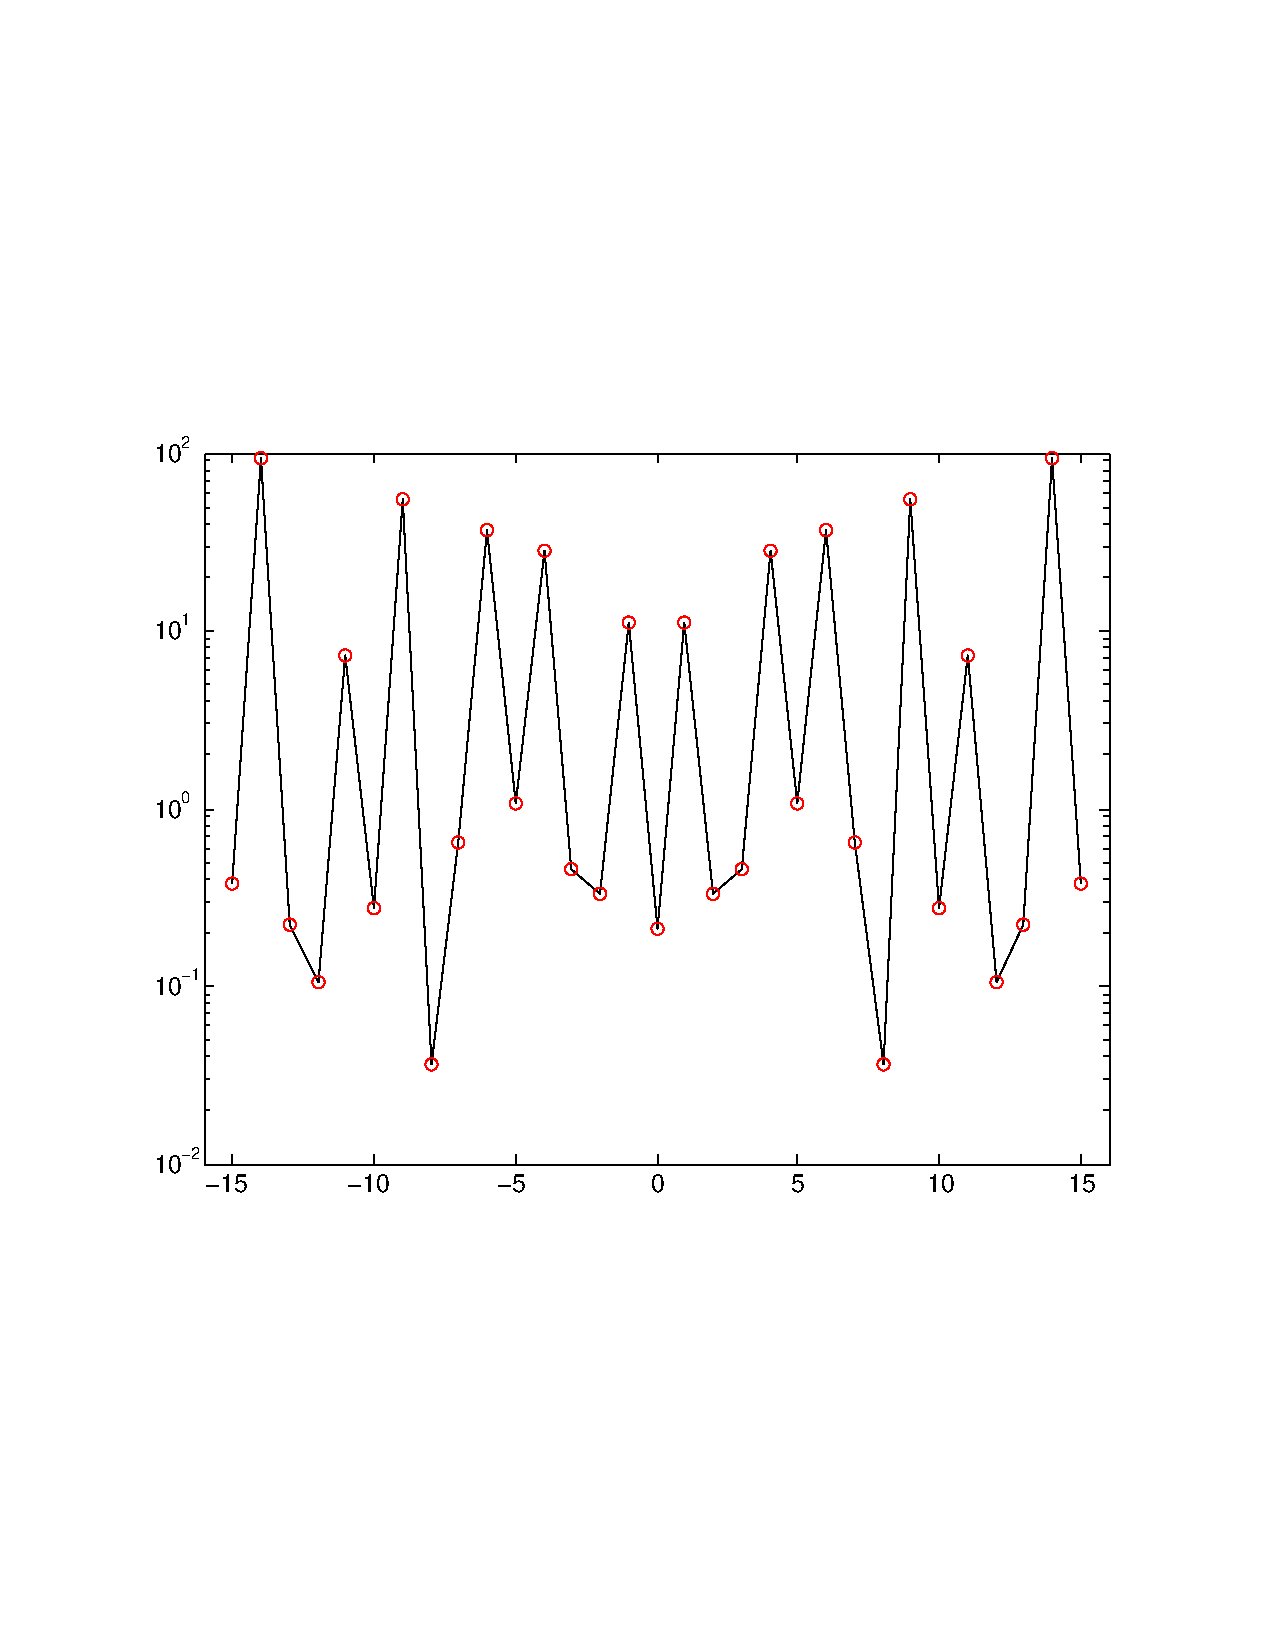
\includegraphics[scale=0.25]{figs/tracAliasingUp4N32}
  \end{tabular}
  \todo{These figs will need to be moved to tikz}
  \mcaption{Top: The spectrum of the exact traction jump (black line)
  and the approximate traction jump at $N=8, 16, 32$ points (red
  circles) for the flower geometry.  Middle: The spectrum of the exact
  traction jump (black line) and the approximate traction jump at $N=8,
  16, 32$ points (red circles) for the flower geometry.  The traction
  jump is computed at $2N$ points, and then spectrally projected to $N$
  points.  Bottom: The spectrum of the exact traction jump (black line)
  and the approximate traction jump at $N=8, 16, 32$ points (red
  circles) for the flower geometry.  The traction jump is computed at
  $4N$ points, and then spectrally projected to $N$
  points.}{f:tracAliasingError}
\end{figure}



\begin{table}[htpb]
\centering
\begin{tabular}{c|cc|cc|cc|cc|}
 & \multicolumn{2}{c|}{$1 \times$} 
 & \multicolumn{2}{c|}{$2 \times$}
 & \multicolumn{2}{c|}{$4 \times$}
 & \multicolumn{2}{c|}{$8 \times$} \\
 $N$ & Low & High & Low & High & Low & High & Low & High \\
 \hline
 8  & 4.56e-1  & 5.55e-1
    & 1.35e-1  & 1.54e-1
    & 3.57e-3  & 3.80e-3
    & 1.17e-5  & 1.03e-5
    \\
 12 & 2.59e-1  & 4.26e-1
    & 2.43e-2  & 3.76e-2
    & 4.52e-5  & 6.39e-5
    & 3.35e-8  & 6.68e-8
    \\
 16 & 1.49e-1  & 3.31e-1
    & 3.75e-3  & 8.55e-3
    & 4.42e-7  & 9.52e-7
    & 8.81e-11 & 3.63e-10
    \\
 24 & 3.64e-1  & 1.69e-1
    & 6.22e-5  & 3.54e-4
    & 2.92e-11 & 1.63e-10
    & 3.21e-15 & 3.09e-14
    \\
 32 & 7.80e-3  & 8.00e-2
    & 8.71e-7  & 1.34e-5
    & 6.83e-15 & 5.73e-15
    & 9.74e-15 & 5.20e-14
\end{tabular}
\mcaption{The errors for approximating the traction jump for the
elliptical geometry at different upsampling
rates.}{t:ellipseTractionErrors}


\begin{tabular}{c|cc|cc|cc|cc|}
 & \multicolumn{2}{c|}{$1 \times$} 
 & \multicolumn{2}{c|}{$2 \times$}
 & \multicolumn{2}{c|}{$4 \times$}
 & \multicolumn{2}{c|}{$8 \times$} \\
 $N$ & Low & High & Low & High & Low & High & Low & High \\
 \hline
 8  & 9.92e-1 & 9.76e-1
    & 9.82e-1 & 9.53e-1
    & 9.71e-1 & 9.32e-1
    & 9.70e-1 & 9.29e-1
    \\
 12 & 9.92e-1 & 9.67e-1
    & 9.81e-1 & 9.37e-1
    & 9.74e-1 & 9.21e-1
    & 9.74e-1 & 9.20e-1
    \\
 16 & 9.75e-1 & 1.05e0
    & 9.66e-1 & 1.09e0
    & 9.64e-1 & 1.10e0
    & 9.64e-1 & 1.10e0
    \\
 24 & 1.48e-1 & 6.60e-1
    & 4.81e0  & 2.00e0
    & 8.11e0  & 8.19e0
    & 1.62e1  & 1.24e1
    \\
 32 & 9.97e-1 & 7.39e-1
    & 6.34e-1 & 2.73e-1
    & 8.01e-2 & 3.61e-2
    & 2.43e-2 & 6.05e-3
    \\
 48 & 5.51e-1 & 3.04e-1
    & 1.76e-1 & 1.47e-1
    & 5.13e-3 & 3.65e-3
    & 2.37e-4 & 1.40e-4
\end{tabular}
\mcaption{The errors for approximating the traction jump for the curly
geometry at different upsampling rates.}{t:curlyTractionErrors}

\begin{tabular}{c|cc|cc|cc|cc|}
 & \multicolumn{2}{c|}{$1 \times$} 
 & \multicolumn{2}{c|}{$2 \times$}
 & \multicolumn{2}{c|}{$4 \times$}
 & \multicolumn{2}{c|}{$8 \times$} \\
 $N$ & Low & High & Low & High & Low & High & Low & High \\
 \hline
 8  & 1.11e0  & 1.75e1
    & 1.26e0  & 2.51e0
    & 1.37e0  & 3.87e3
    & 1.38e0  & 4.13e0
    \\
 12 & 1.27e0  & 6.50e-1
    & 2.61e0  & 4.16e-1
    & 5.49e0  & 9.85e-1
    & 7.40e0  & 1.84e0
    \\
 16 & 9.01e-1  & 5.07e-1
    & 4.52e-1  & 2.53e-1
    & 3.03e-2  & 1.60e-2
    & 4.07e-5  & 2.15e-5
    \\
 24 & 5.85e-1  & 5.20e-1
    & 1.34e-1  & 1.23e-1
    & 1.19e-3  & 1.09e-3
    & 1.02e-8  & 8.85e-9
    \\
 32 & 2.68e-1  & 3.79e-1
    & 1.71e-2  & 3.50e-2
    & 2.30e-5  & 4.61e-5
    & 3.97e-12 & 7.07e-12
    \\
 48 & 1.25e-1  & 2.57e-1
    & 1.11e-3  & 2.46e-3
    & 9.10e-9  & 1.89e-8
    & 2.99e-14 & 6.82e-14
\end{tabular}
\mcaption{The errors for approximating the traction jump for the flower
geometry at different upsampling rates.}{t:flowerTractionErrors}



\end{table}


%%%%%%%%%%%%%%%%%%%%%%%%%%%%%%%%%%%%%%%%%%%%%%%%%%%%%%%%%%%%%%%%%%%%%%%%%
%\subsection{Aliasing and filtering}
%\begin{itemize}
%  \item Equi-distribution in arclength is key
%  \item Multiplication is straight forward using the three-halves rule
%  \item Fourier differentiation and exponentiation requires some work to
%  decide on optimal upsampling rates.
%\end{itemize}
%
%At low resolutions, aliasing can become an issue.  That is, when
%performing operations on periodic functions such as $(\sigma \xx_{s})$,
%the frequencies that are beyond the Nyquist frequency will be aliased
%into lower frequencies.  One method to reduce or eliminate aliasing is
%to use appropriate levels of upsampling.
%
%When computing the product $fg$ of two periodic functions, both
%represented by $N$ points (or frequencies), a standard approach is to
%upsample both $f$ and $g$ to $1.5 N$ points, perform the
%multiplication, and then zero all the frequencies except the first
%$N$.  This has the effect of completely eliminating the aliasing as is
%illustrated in Figure~\ref{} \todo{Figure showing aliasing here}.
%
%Unfortunately, our governing equations involve operations that are much
%more complicated than the simple quadratic operation.  For instance,
%given a closed curve $\xx$, we need to compute the arclength derivative
%$\ff_{s}$ of many different functions $\ff$.  This is equivalent to
%computing
%\begin{align}
%  \frac{1}{\|\xx'(\theta)\|}\frac{d\ff}{d\theta}.
%\end{align}
%In general, our discretization is not equispaced in arclength, and,
%therefore, $\|\xx'(\theta)\|$ is not constant.  Therefore, we need to
%compute the quotients of periodic functions.  Here consider computing
%the most simple quotient $g = 1/f$ where $f$ is periodic and $f > 0$.
%Unfortunately, even if $f$ is band-limited, $g$, in general, is not.
%For instance
%\begin{align}
%  \frac{1}{\cos(\theta) + 2}
%\end{align}
%is not band-limited, and 52 modes are required before machine precision
%is achieved (Figure~\ref{}), even though the function $f$ only has
%three frequencies (-1, 0, and 1). \todo{Plot spectrum of this
%function}.  Therefore, completely removing the aliasing is impossible,
%and some error will inevitably be introduced.
%
%The final operation that we must consider are powers of periodic
%functions.  For instance, the square-root of periodic functions are
%required when computing the norm of a vector
%\begin{align}
%  \| \xx \| = \sqrt{x_{1}(\theta)^{2} + x_{2}(\theta)^{2}}.
%\end{align}
%As is the case with division of periodic functions, taking powers of a
%band-limited periodic function can result in a function that is not
%band-limited.  For instance, consider $g(\theta) = f^{1/2} =
%(\cos(\theta) + 2)^{1/2}$.  Again, $f$ is band-limited, but $g$
%requires 46 modes before machine precision is achieved (Figure~\ref{}).
%
%When computing products of periodic functions, we use the
%three-halves-rule to completely eliminate aliasing.  To remain
%consistent, we use this same upsampling rule for quotients and powers
%of periodic functions.  While this does not completely eliminate the
%aliasing, it does reduce it.
%
%Even with aliasing, it is possible that errors in the high frequencies
%can cascade and result in an unstable method.  Therefore, at low
%resolutions, we will also be considering a filtering strategy.  The
%technique is to filter all $N$-point periodic functions by assigning a
%value of zero to all modes whose absolute value is greater than $N/3$.


%%%%%%%%%%%%%%%%%%%%%%%%%%%%%%%%%%%%%%%%%%%%%%%%%%%%%%%%%%%%%%%%%%%%%%%%
\subsection{Local corrections to area and length}
\label{s:localCorrect}
When a simulation has a long time horizon, the accumulation of errors in
a vesicles area and length often leads to instabilities.  We have
introduced an adaptive time stepping method~\cite{qua:bir2014b} that
allows a user to specify a tolerance for the time horizon a priori.
However, this only controls time stepping error.  Other sources of
errors, including spatial errors, GMRES tolerance, and issues with
conditioning can also lead to an accumulation of error.  Therefore, we
introduce a technique where the vesicle's shape is corrected at each
time step.  This is achieved through a constrained optimization problem,
where the constraints require the vesicle to have the correct area and
length, both of which are conserved quantities.  

Suppose that a vesicle initially has area $A_{0}$ and length $L_{0}$,
and that a time integrator is used to form a solution $\tilde{\xx}$ at
time $t$.  We make a local correction to the vesicle's shape by using
sequential quadratic programming (SQP) to solve
\begin{align*}
  \min_{\substack{A(t) = A_{0} \\ L(t) = L_{0}}} 
    \|\xx(t) - \tilde{\xx}(t)\|^{2},
\end{align*}
for a new shape $\xx(t)$.  In Section~\ref{s:results}, we show that this
correction is essential for suspensions with long time horizons and high
volume fractions.


%%%%%%%%%%%%%%%%%%%%%%%%%%%%%%%%%%%%%%%%%%%%%%%%%%%%%%%%%%%%%%%%%%%%%%%%
\subsection{Equi-distribution in arclength}
In interfacial dynamics, time stepping and other sources of error can
cause Lagrangian tracker points to cluster.  This leads to instabilities
when computing high-order derivatives, such as the one that arises when
a Helfrich energy is used.  Therefore, we are interested in strategies
that maintain an equi-distribution of the points in arclength.  In
vesicle suspensions, the local inextensibility constraint enforces that
the distance between successive discretization points remains fixed.
However, due to numerical errors, points may begin to cluster (see
Figure~\ref{f:shearEquiArclength}).  Given a shape
\begin{align*}
  \xx(\theta) = \sum_{n=1}^{N} \hat{\xx}_{n} e^{in\theta},
\end{align*}
we find the $N$ values, $\theta_{j} \in [0,2\pi)$, $j=1,\ldots,n$ such
that
\begin{align}
  L(\theta_{j}) = \int_{0}^{\theta_{j}} |\xx(\omega)| d\omega = 
    (j-1)\frac{L}{N}, \quad j=1,\ldots,N,
  \label{e:equiarclength}
\end{align}
where $L = L(2\pi)$ is the total length of the vesicle.  $L(\theta)$ is
spectrally evaluated at the $N$ equispaced points $(j-1)\frac{2\pi}{N}$,
$j=1,\ldots,N.$  Then, equation~\eqref{e:equiarclength} is solved with a
local spline interpolant.  Since the points $\theta{j}$ are not
equi-distributed, a uniform FFT can not be used to construct $\xx$.
Since we are interested in small values of $N$, we opt to use the direct
$\bigO(N^{2})$ algorithm rather than a non-uniform FFT which could
require $\bigO(N\log N)$ operations, but with potentially a large
constant.


%%%%%%%%%%%%%%%%%%%%%%%%%%%%%%%%%%%%%%%%%%%%%%%%%%%%%%%%%%%%%%%%%%%%%%%%
\subsection{Adaptive time stepping and spectral deferred correction}
In~\cite{qua:bir2014b, qua:bir2014c}, we developed a high-order adaptive
time integrator.  The time step size depends on the amount of error
committed in area and length at each time step, and high-order accuracy
is achieved through spectral deferred correction (SDC) sweeps.
Unfortunately, at low resolutions and low accurate FMMs and GMRES
tolerances, the time stepping error does not always dominate.
Therefore, we do not expect to achieve second-order or higher-order
accuracy in time.  However, we can interpret SDC as an iterative method
that converges to the fully-implicit collocations scheme.  In
particular, the SDC algorithm converges to the solution of a quadrature
formula of
\begin{align}
  \xx(t+\Delta t) = \xx(t) + \int_{t}^{t+\Delta t} \vv(\xx(\tau)) d\tau,
  \label{e:picardFormulation}
\end{align}
where $\vv$ is the velocity of the vesicle.

For the quadrature formula of the Picard
integral~\eqref{e:picardFormulation}, we use the first-order method
\begin{align*}
  \int_{t}^{t+\Delta t} \vv(\xx(\tau))d\tau = \Delta t v(\xx,t+\Delta t).
\end{align*}
In this manner, we only obtain first-order accuracy. \todo{need a good
reason to do this}.

In order to build in adaptivity, we only accept the current solution if
$E(t+\Delta t) < \epsilon \Delta t$, where $E$ is the maximum error in area
and length.  Then, owning to the first-order discretization, the new
time step size is
\begin{align*}
  \Delta t_{\mathrm{new}} = \left(\frac{E(t) }{}  \right).
  \todo{not sure how this works since we correct vesicle shape}
\end{align*}
The safety parameters are chosen based on experiments, and for the low
resolution simulations of interest, we have found that $\alpha=$
$\beta_{\mathrm{up}}=$, and $\beta_{\mathrm{down}}=$ give an acceptable
balance between rejected and accepted time steps.

Finally, after a time step size has been accepted, the vesicle shape is
corrected by fixing the area and length as is described in
Section~\ref{s:localCorrect}


%%%%%%%%%%%%%%%%%%%%%%%%%%%%%%%%%%%%%%%%%%%%%%%%%%%%%%%%%%%%%%%%%%%%%%%%
\subsection{Near-singular integration}
Not sure if anything new will have to be done here to handle
nearly-touching very coarse representations of the vesicles.
One thing we can adjust is the number of interpolation points used off
of the boundary to do the interpolation.  Hopefully 2 plus the boundary
point would be enough.
\todo{Plots showing that the proposed algorithm is fine.  Compare with
and without anti-aliasing?}
\todo{Nothing is moving.  Just two (or more) vesicles are very close to
one another}


%%%%%%%%%%%%%%%%%%%%%%%%%%%%%%%%%%%%%%%%%%%%%%%%%%%%%%%%%%%%%%%%%%%%%%%%
\subsection{Accuracy of the far field}
Here we investigate the treatment of the far field.  Some
groups~\cite{} (including ours) use an implicit or semi-implicit method
to discretize the interactions between distinct vesicles.  However,
many groups~\cite{} treat these interactions explicitly.  Here we
discuss a method that allows us to investigate the significance of how
inter-vesicle interactions are discretized.

Rather than changing how we discretize vesicle-vesicle interactions, we
continue to use the semi-implicit discretization from our previous
work~\cite{qua:bir2014a}, and then adjust the tolerance of the fast
multipole method.  This has the effect of adjusting the accuracy of the
far field (V-lists).  Since the interaction due to the near field
(U-list) is treated directly, adjusting the FMM tolerance does not
effect the interaction with sufficiently close vesicles.
\todo{Examples to look at are extensional and shear with large volume
fraction}



